\chapter{Gradient-accelerated Inference for Diverse Counterexamples}\label{ch:corl}

In Chapters~\ref{ch:rss} and~\ref{ch:iros}, we introduce local gradient-based optimization methods for design, using standard optimization and adversarial verification-guided optimization. As discussed at the end of Chapter~\ref{ch:iros}, there are a few drawbacks inherent to local methods.

\begin{enumerate}
    \item \textbf{Risk of local minima: } Local gradient-based optimizers are greedy and prone to getting stuck in local minima. This risk is particularly important in safety-critical use cases, since converging to a counterexample that is far from the true worst-case might lead us to falsely believe that a design is safe.
    \item \textbf{Lack of diversity in adversarial examples: } When verifying a system, it is important to consider a diverse set of failure modes. However, optimization-based approaches have difficulty balancing exploration with exploitation; nearby solutions will typically converge to the nearest local optimum.
    \item \textbf{Sensitivity to gradient quality: } Many robotic systems, particularly those involving contact or vision, have dynamics that are not differentiable everywhere, as we assumed in previous chapters. Even when these dynamics are smoothed, there are still regions where the gradients can be poorly conditioned (i.e. arbitrarily large) or flat, which will cause a gradient-based optimizer to diverge or get stuck.
\end{enumerate}

% TODO Emphasize vision in the loop and what we will be able to do if we figure these things out

In this chapter, we address these drawbacks by re-framing the counterexample-guided optimization problem from Chapter~\ref{ch:iros} as a Bayesian inference problems, which we then solve using gradient-accelerated Markov Chain Monte Carlo (MCMC) methods. We demonstrate empirically how this Bayesian inference framework provides improved performance (in both convergence speed and solution quality) over both gradient-based and gradient-free optimization methods, and we provide a theoretical analysis to support these empirical observations. This chapter is based in part on the author's published work in~\cite{dawsonBayesianApproachBreaking2023}.

\section{Related work}

% TODO Move this to the background chapter
Our work builds on a rich literature of different verification and testing techniques, which we review here.

\paragraph{Model-based verification}

Early work on model based verification relied on logical models to search for failures using satisfiability (SAT) solvers~\cite{dekleerDiagnosingMultipleFaults1987,benardRemoteAgentExperiment2000}. The computational expense of SAT, which prevented these methods from scaling to high-dimensional problems, motivated the development of more recent approaches using mathematical dynamics models and tools like reachability analysis~\cite{annpureddySTaLiRoToolTemporal2011} and optimal control~\cite{chouUsingControlSynthesis2018} to identify counterexamples. The challenge in applying all of these methods is that it is often difficult (or impossible) to construct a symbolic model of the system under test (e.g. when vision is involved). In this work, our aim is to preserve the interpretability of model-based verification without relying on a symbolic model. Instead, we develop a simulation-based approach using automatic differentiation (when available) to accelerate the search for counterexamples. Simulators are widely used in robotics, and recent work on differentiable simulation and rendering has made gradients available for a range of scenarios~\cite{amosOptNetDifferentiableOptimization2017,belubute_peres_lcp_physics,Jakob2020DrJit,jainAnalyzingImprovingNeural2020,huDiffTaichiDifferentiableProgramming2019,zhongGuidedConditionalDiffusion2022,dawsonCertifiableRobotDesign2022,dawsonRobustCounterexampleguidedOptimization2022b}.

\paragraph{Adversarial testing}

A common approach in the falsification literature is adversarial optimization, which formulates the search for counterexamples as a two-player game between the system designer and the environment~\cite{dawsonRobustCounterexampleguidedOptimization2022b,dontiAdversariallyRobustLearning2021,yaghoubiGrayboxAdversarialTesting2018,corsoSurveyAlgorithmsBlackBox2021,xuSafeBenchBenchmarkingPlatform2022,riedmaierSurveyScenarioBasedSafety2020,okellyScalableEndtoEndAutonomous2018,corsoAdaptiveStressTesting2019,wangAdvSimGeneratingSafetyCritical2021,sunCornerCaseGeneration2021,zhongGuidedConditionalDiffusion2022,corsoInterpretableSafetyValidation2020a,zhangAdversarialRobustnessTrajectory2022,hanselmannKINGGeneratingSafetyCritical2022a}. Adversarial methods have been developed in both model-based and model-free contexts, where the main distinction is that the former assume access to gradients. Gradient-based adversarial methods have demonstrated impressive sample efficiency~\cite{dawsonRobustCounterexampleguidedOptimization2022b,dontiAdversariallyRobustLearning2021}, but the drawback is that they rely on local gradient ascent to search for counterexamples, typically yielding only a single adversarial counterexample that may be only locally optimal. Moreover, existing gradient-based methods cannot handle systems with visual feedback. \cite{hanselmannKINGGeneratingSafetyCritical2022a} find that skipping the rendering step during backpropagation is sufficient for gradient-based failure-case generation, but this method is not able to repair visual-feedback policies. \cite{sinhaNeuralBridgeSampling2020} learn a proxy model for the end-to-end dynamics, including a vision-based policy, but end-to-end proxy modeling is generally not applicable to rare-event generation, since it is difficult to include enough failure examples in the training data for the proxy model.
%
On the other hand, gradient-free methods reduce the risk of getting stuck in local optima and support vision in the loop, but they require additional computation and struggle to scale to high-dimensional search spaces. In contrast, in this work we develop a probabilistic gradient-based approach, using sample-efficient gradient-based sampling algorithms to avoid local minima and scale to high dimensional search spaces, and using differentiable rendering to support visual feedback systems. We also provide a gradient-free variant of our method for use in cases when a differentiable simulator is not available.

\paragraph{Inference}

Our probabilistic approach builds off of prior work on inference as a verification tool. \cite{okellyScalableEndtoEndAutonomous2018} propose an end-to-end verification tool for autonomous vehicles based on gradient-free adaptive importance sampling. \cite{zhouRoCUSRobotController2021} use gradient-free Markov Chain Monte Carlo (MCMC) to find counterexamples. \cite{sinhaNeuralBridgeSampling2020} and \cite{deleckiModelbasedValidationProbabilistic2023a} use gradient-based MCMC to estimate the risk of failure and find counterexamples, respectively.
%
These prior works are focused only on predicting failure modes; they are not able to improve the system (e.g. by re-optimizing the controller) to fix these failures once they have been discovered. Our method aims to fill this gap by combining failure mode prediction and repair, exploiting the duality between these problems to efficiently search for both a diverse set of counterexamples and updates to the system's policy or design that reduces the severity of those failures.

\section{From optimization to inference}

To motivate the switch from optimization to inference, consider the toy example of optimizing the cost landscape shown on the left in Fig.~\ref{ch:corl:fig:toy_example}. This cost function has local minima at $x = -0.544$ (marked with a square) and $x = 0.919$ (the true global optimum, marked with a circle). If initialized with $x < 0$, a local gradient-based optimizer will naturally converge to the sub-optimal local minimum at $x = -0.544$, missing the global minimum. We can see this behavior in Fig.~\ref{ch:corl:fig:toy_example_convergence}, which plots the convergence of gradient-based optimization with 5 different random starting positions $x\sim\cN(-1.5, 0.1)$. All 5 runs converge to the suboptimal local minimum at $x = -0.544$.

To avoid getting stuck in this local minimum, we can convert this optimization problem into an inference problem; i.e. sampling from the unnormalized probability density:
\begin{align*}
    \argmin_x U(x) \quad \implies \quad x \sim p(x) \propto e^{-U(x)}
\end{align*}
%
This unnormalized distribution is shown on the right in Fig.~\ref{ch:corl:fig:toy_example}. We can see that the distribution is bimodal, with a peak at the suboptimal local minimum and a larger peak at the global minimum. By sampling from this distribution, we can find the global minimum with high probability (this is the so-called \textit{Optimization as Inference} perspective~\cite{maSamplingCanBe2019,levineReinforcementLearningControl2018a}). In practice, we can approximately sample from this distribution using Markov Chain Monte Carlo (MCMC) methods, which we will discuss in more detail shortly. The benefit of these methods is that they balance exploring different regions of the distribution with exploiting high-likelihood areas; we can see this behavior in Fig.~\ref{ch:corl:fig:toy_example_convergence}, which shows the convergence of Metropolis-adjusted Langevin (MALA) MCMC, a gradient-based inference method, on the same cost landscape over 5 different random seeds. MALA is able to find the global minimum with high probability, while gradient-based optimization gets stuck in the local minimum.

\begin{figure}[tb]
    \centering
    \begin{subfigure}[b]{\linewidth}
        \centering
        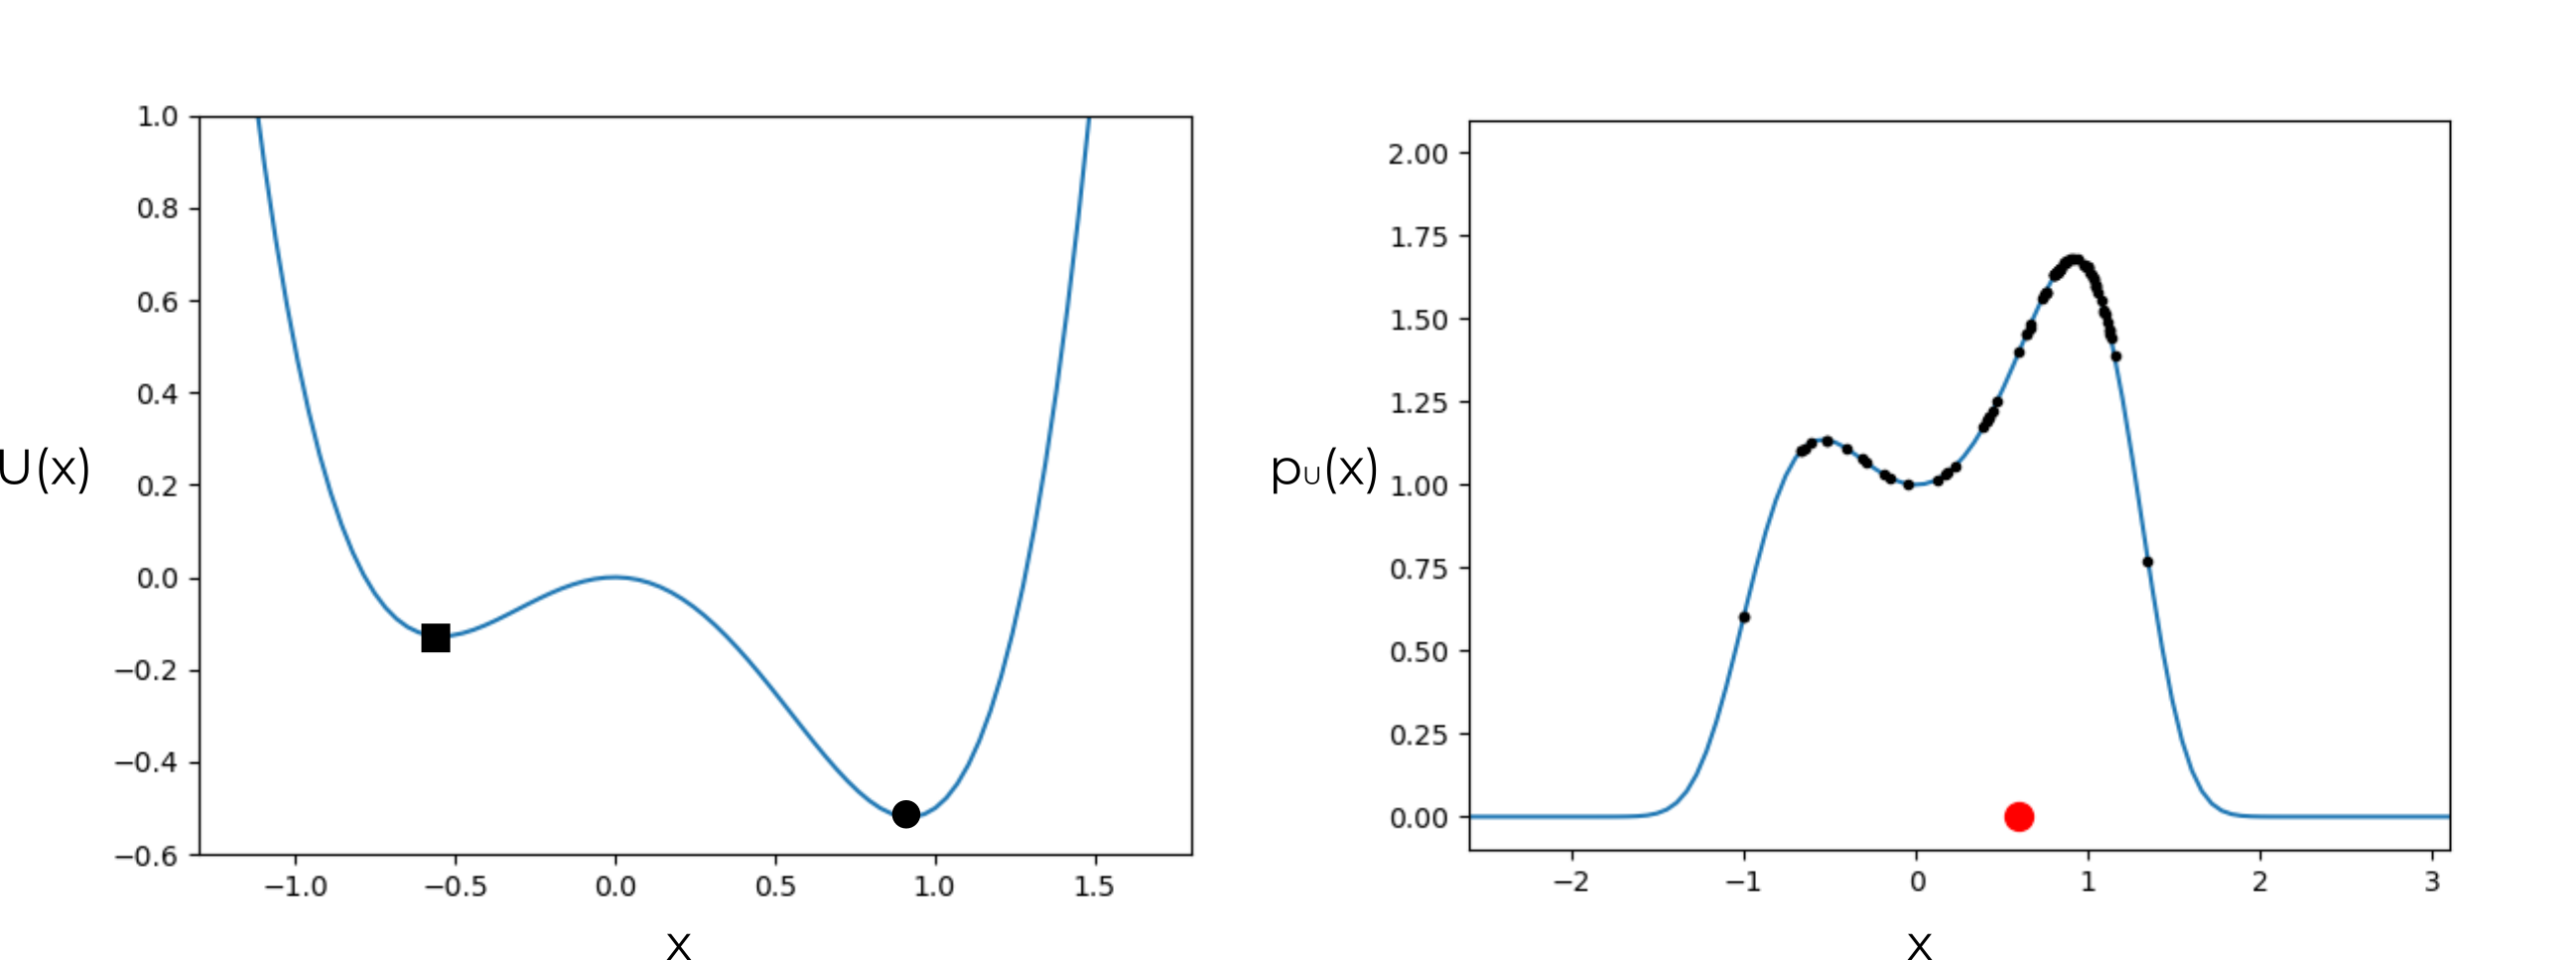
\includegraphics[width=0.9\linewidth]{images/global_methods/sampling_as_optimization.png}
        \caption{Left: a simple bimodal cost landscape $U(x) = x^4 - 0.5 x^3 - x^2$, with a locally optimal solution at $x\approx -0.544$ and a global optimum at $x\approx 0.919$. Right: the corresponding unnormalized likelihood $p(x) \propto e^{-U(x)}$, showing samples drawn from this distribution (black dots) and the average of 100 samples (red dot).}
        \label{ch:corl:fig:toy_example}
    \end{subfigure}

    \begin{subfigure}[b]{\linewidth}
        \centering
        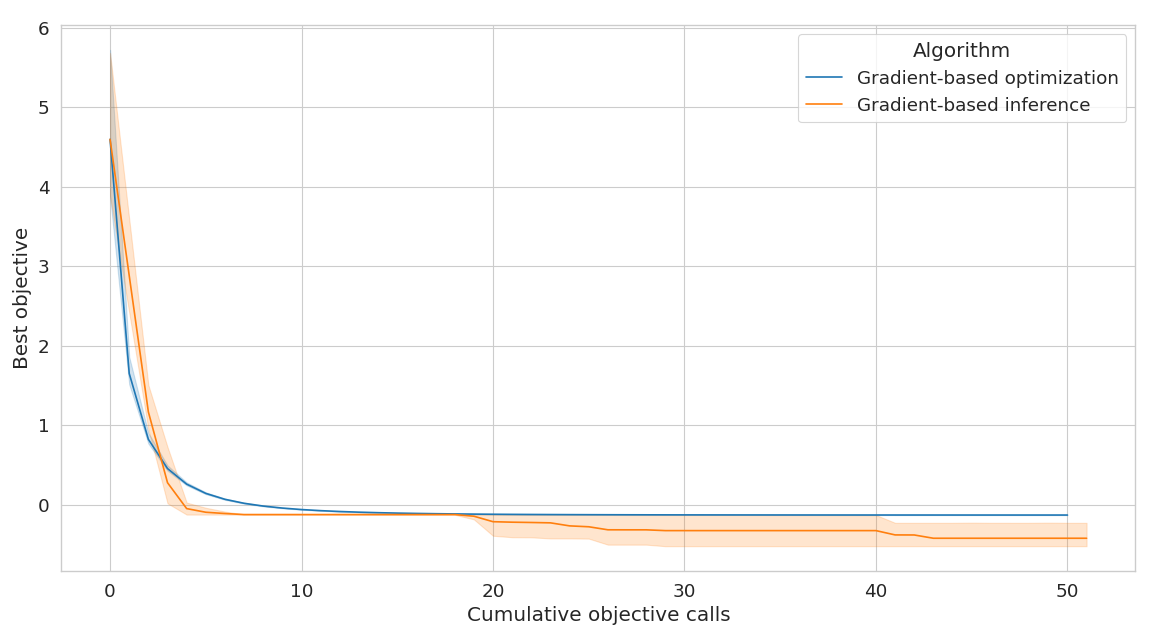
\includegraphics[width=0.7\linewidth]{images/global_methods/double_well_gd_mala.png}
        \caption{Convergence of gradient-based optimization and inference (Metropolis-adjusted Langevin) on the double-well cost landscape from Fig.~\ref{ch:corl:fig:toy_example}, showing how the optimization method gets stuck in a local minimum while the inference method is able to escape and find the global minimum.}
        \label{ch:corl:fig:toy_example_convergence}
    \end{subfigure}
\end{figure}

A wide variety of MCMC algorithms exist to sample from arbitrary non-normalized probability distributions~\cite{geyerIntroductionMarkovChain2011}; common variants include Random-walk Metropolis-Hastings (RMH), Hamiltonian Monte Carlo (HMC), unadjusted Langevin (ULA), and MALA. RMH is gradient-free, while HMC, ULA, and MALA are gradient-based. MALA, which can be seen as a single-step version of HMC, is outlined in Algorithm~\ref{ch:corl:alg:mala}. Like all MCMC algorithms, it defines a Markov chain with a transition rule designed to preserve the so-called detailed balance condition, which ensures that the stationary distribution of the Markov chain is the same as the target density (see~\cite{geyerIntroductionMarkovChain2011,aiama} for a more complete introduction). MALA defines a transition rule that begins by proposing a candidate state in line~\ref{ch:corl:alg:mala:step} using a gradient-driven drift term and a Gaussian diffusion term. The candidate state is accepted with probability $P_{accept}$ in line~\ref{ch:corl:alg:mala:mh}, which is proportional to the ratio of the target density at the candidate and current states. If the candidate state is accepted, it becomes the new current state; otherwise, the current state is repeated. The algorithm is run for $K$ steps, and the final state is returned as the sample from the target density.

\begin{algorithm}
    \caption{Metropolis-adjusted Langevin algorithm (MALA,~\cite{maSamplingCanBe2019,robertsLangevinDiffusionsMetropolisHastings2002})\label{ch:corl:alg:mala}}
    \DontPrintSemicolon
    \KwInput{Initial $x_0$, steps $K$, stepsize $\epsilon$, density $p(x)$.}
    \KwOutput{A sample drawn from $p(x)$.}
    \For{$i = 1, \ldots, K$}
    {
    Sample $\eta \sim \cN(0, 2\epsilon I)$ \Comment{Gaussian noise}\;
    $x_{i+1} \gets x_i + \epsilon \nabla \log p(x_i) + \eta$ \Comment{Propose next state}\;\label{ch:corl:alg:mala:step}
    $P_{accept} \gets \frac{p(x_{i+1}) e^{-||x_i - x_{i+1} - \epsilon \nabla \log p(x_{i+1})||^2 / (4\epsilon)}}{p(x_{i}) e^{-||x_{i+1} - x_{i} - \epsilon \nabla \log p(x_{i})||^2 / (4\tau)}}$ \;
    With probability $1 - \min(1, P_{accept})$:
    \hspace{2em}$x_{i+1} \gets x_{i}$ \Comment{Accept/reject proposal}\;\label{ch:corl:alg:mala:mh}
    }
    \KwRet{$x_K$}
\end{algorithm}

We have shown how transitioning from gradient-based optimization to inference (in particular, gradient-based inference using MALA) addresses the first drawback identified at the start of this chapter (the risk of getting stuck in local minima). Next, we will discuss how gradient-based inference also addresses the other two drawbacks (the difficulty of sampling diverse failure modes and sensitivity to gradient quality).

\subsection{Sampling diverse solutions}

MCMC sampling methods provide a principled means for balancing exploration and exploitation, and so they are well-suited to problems with multiple modes (particularly when the modes are close together in the search space). However, although MCMC methods enjoy good asymptotic guarantees, including ergodicity and convergence to the target distribution in the inifinite-sample limit, any finite-sample implementation will struggle to explore a highly multi-modal target distribution if the modes are well separated (any finite MCMC run will be biased towards the modes near its starting point). A family of algorithms known as sequential Monte Carlo (SMC) algorithms exist to solve this problem by smoothly interpolating between a sequence of distributions, starting from a simple distribution (e.g., a Gaussian) and ending at the target distribution~\cite{chopinIntroductionSequentialMonte2020}. SMC algorithms are particularly useful for inference problems with multiple modes, since they can be used to sample from the target distribution in a way that is less biased by the initialization. In the following section, we will discuss how SMC can be applied to sample diverse solutions (both failure modes and designs) for practical autonomous system design and verification problems.

\subsection{Sensitivity to gradient quality}% TODO include discussion of rendering

As discussed at the start of this chapter and in prior work~\cite{suhDifferentiableSimulatorsGive2022,suh2021_bundled_gradients}, many practical robotics problems involve non-smooth dynamics that may not be differentiable, or even continuous, at all points. For example, dynamics involving rigid body contact are discontinuous at the point when contact is made or broken. Even when these functions can be smoothed, they may still have poorly behaved gradients (e.g. gradients that are either flat or very large). Prior work~\cite{suhDifferentiableSimulatorsGive2022} identifies the ballistic optimization problem shown in Fig.~\ref{ch:corl:fig:ballistic} as a simple problem that illustrates the effect of both flat gradients and discontinuities.

Fig.~\ref{ch:corl:fig:ballistic_convergence} shows the cost of the best solution found by local optimization using gradient descent, inference using MALA (a gradient-based method), and inference using RMH (a gradient-free method), all starting from a point left of the flat region. As expected, we see that gradient descent gets stuck in the flat region, but both inference methods are able to explore the flat region and eventually discover the global optimum. A natural next question is whether and to what extent gradients help the inference methods explore this distribution; to answer this question, we define a high-dimensional version of the ballistic problem that simply runs $N$ instances in parallel (using an $N$-dimensional decision vector with one element for each instance) and returns the total cost across all problems. In low dimensions, there is no discernable difference between the gradient-free and gradient-based inference methods. In higher dimensions $N > 10$, gradient-free RMH does not even reach the flat region where gradient descent gets stuck, while gradient-based MALA converges even in $N=1000$ dimensions.

We attribute this improved performance to three factors. First, the Gaussian diffision term in the MALA proposal allows it to explore the flat region of the cost landscape and eventually find the optimal solution. Second, the accept/reject step provides some robustness to stiff or inaccurate gradients; if a bad gradient causes MALA to propose a state with much higher cost (lower likelihood), then it will likely reject that proposal and try again. Third, the gradient-based drift term in the proposal provides a valuable heuristic for exploring high-dimensional space, where the exponentially decreased volume of the region around the optimal solution makes it difficult to explore using gradient-free methods.

\begin{figure}[t]
    \centering
    \begin{subfigure}[t]{0.6\linewidth}
        \centering
        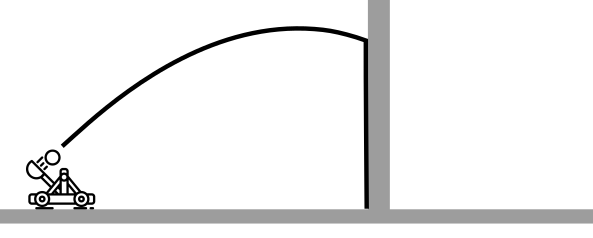
\includegraphics[width=\linewidth]{images/global_methods/ballistic.png}
    \end{subfigure}
    \begin{subfigure}[t]{0.3\linewidth}
        \centering
        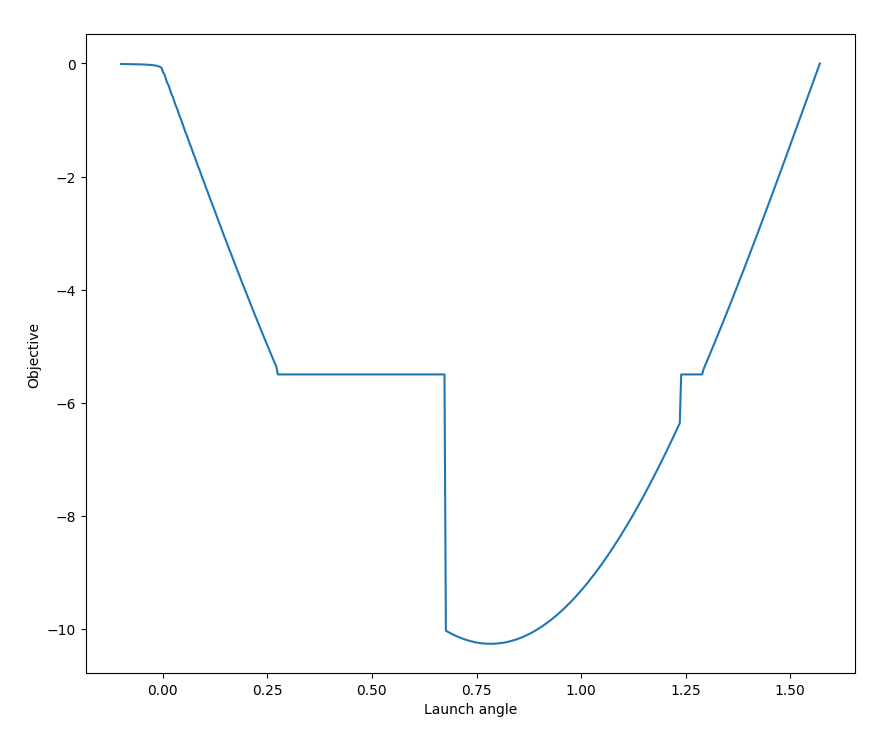
\includegraphics[width=\linewidth]{images/global_methods/ballistic_cost.png}
    \end{subfigure}%
    \caption{Left: the ballistic optimization problem from~\cite{suhDifferentiableSimulatorsGive2022}. Right: the corresponding cost landscape.}
    \label{ch:corl:fig:ballistic}
\end{figure}

\begin{figure}[tb]
    \centering
    \begin{subfigure}[t]{0.24\linewidth}
        \centering
        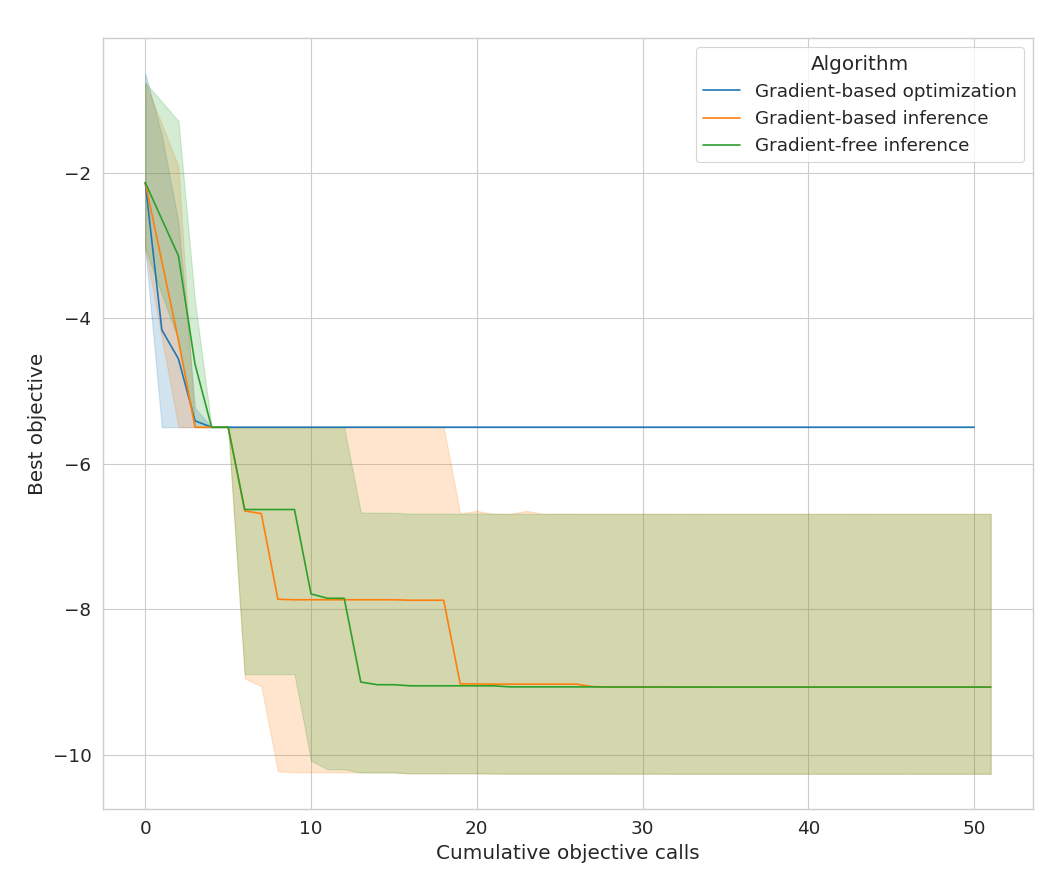
\includegraphics[width=\linewidth]{images/global_methods/ballistic_1.png}
        \caption{$N=1$}
    \end{subfigure}
    \begin{subfigure}[t]{0.24\linewidth}
        \centering
        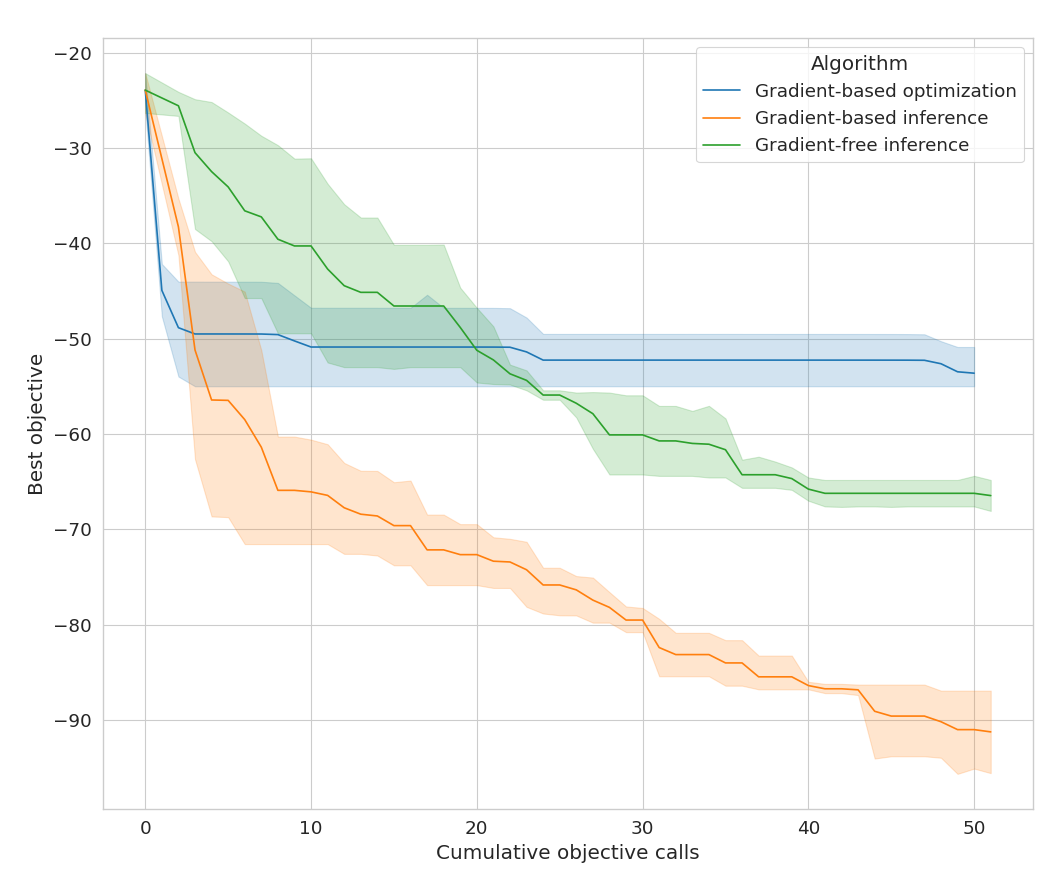
\includegraphics[width=\linewidth]{images/global_methods/ballistic_10.png}
        \caption{$N=10$}
    \end{subfigure}
    \begin{subfigure}[t]{0.24\linewidth}
        \centering
        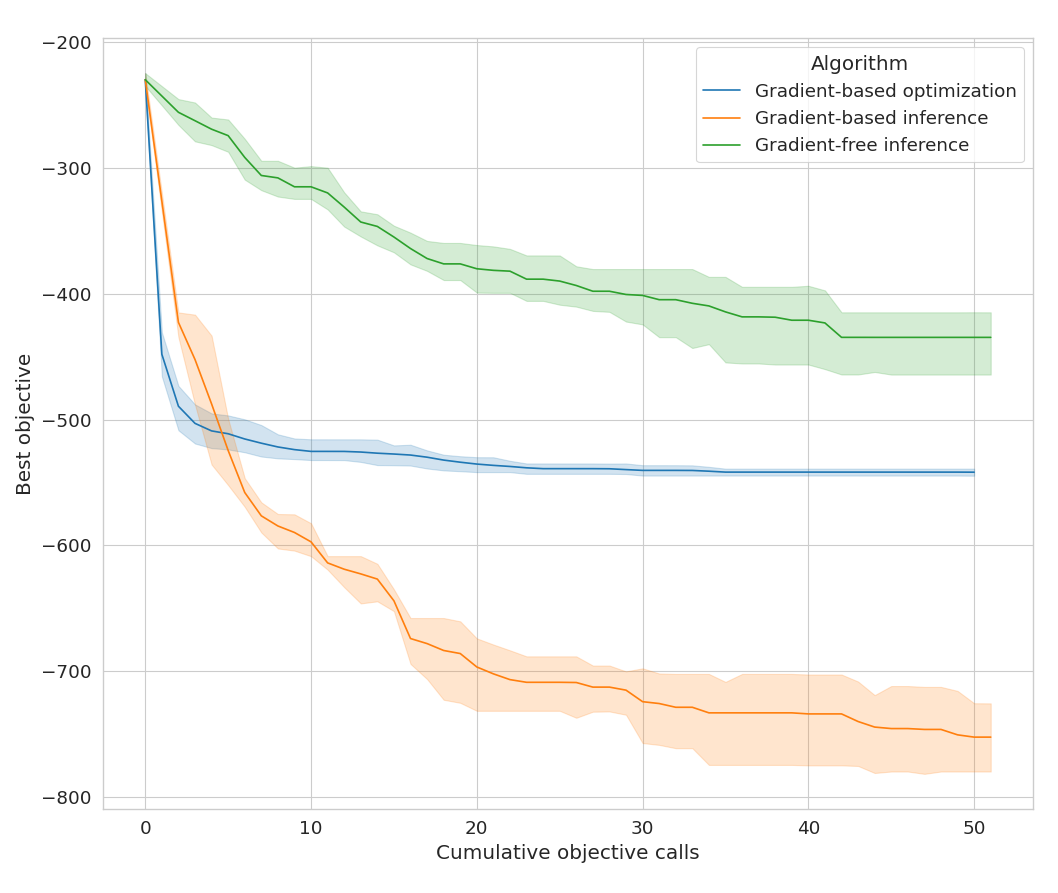
\includegraphics[width=\linewidth]{images/global_methods/ballistic_100.png}
        \caption{$N=100$}
    \end{subfigure}
    \begin{subfigure}[t]{0.24\linewidth}
        \centering
        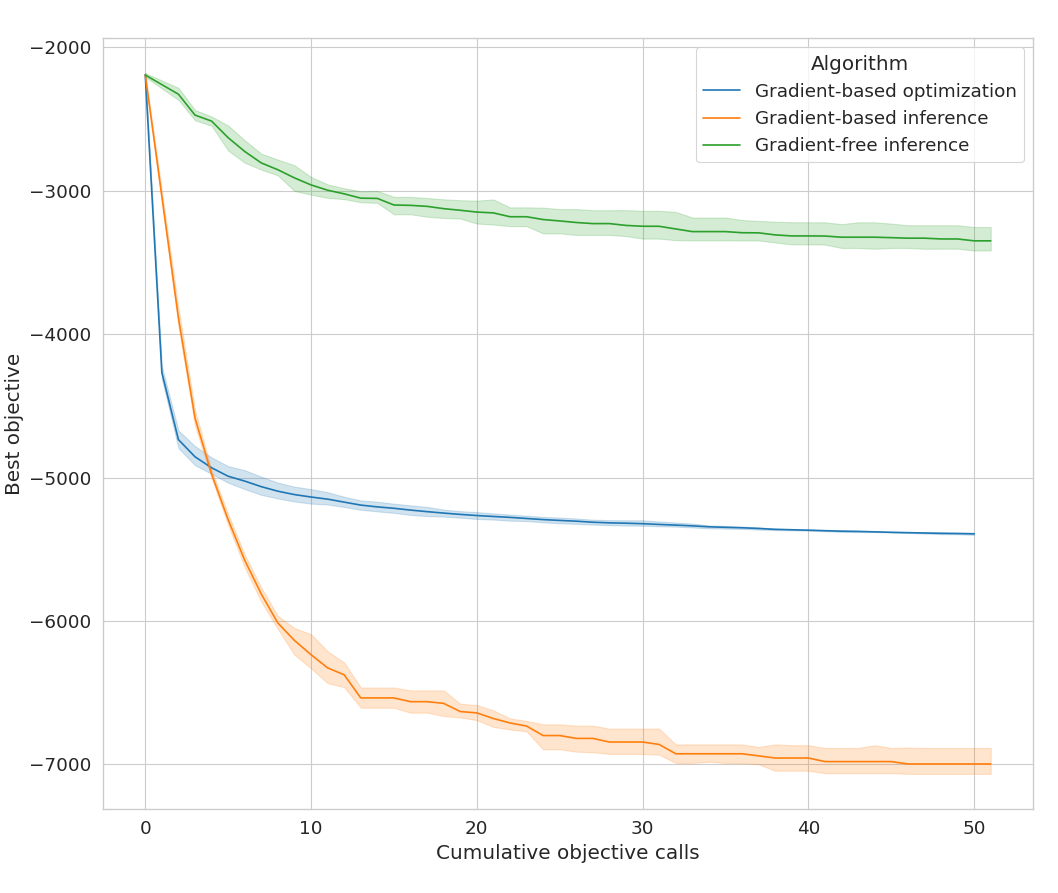
\includegraphics[width=\linewidth]{images/global_methods/ballistic_1000.png}
        \caption{$N=1000$}
    \end{subfigure}
    \caption{Convergence of gradient-based optimization (gradient descent), gradient-based inference (MALA), and gradient-free inference (RMH) on the ballistic cost landscape from Fig.~\ref{ch:corl:fig:toy_example}.}
    \label{ch:corl:fig:ballistic_convergence}
\end{figure}

\subsection{Scaling gradient-based inference to high dimensions}

% TODO include results from additional benchmark problems, maybe even empirical convergence rates as a function of dimension on a number of problems. Introduce theoretical results.

\section{Sampling and repairing diverse failure modes}

% TODO edit for flow

Now that we have motivated the switch from optimization to inference, we will reframe the adversarial optimization from Chapter~\ref{ch:iros} as a sequential inference problem, then demonstrate how we can used gradient-accelerated MCMC sampling (i.e. MALA) to efficiently sample diverse failure modes and find more robust optimized designs.

\subsection{Preliminaries}

Let us define a ``failure mode'' as a set of environmental parameters $\phi$ that induce high cost for given policy parameters $\theta$, i.e. finding multiple solutions $\phi^*(\theta) = \text{find}_\phi J(\theta, \phi) \geq J^*$ for failure threshold $J^*$. In this context, \textit{failure prediction} is the search for such $\phi^*$ given a design $\theta$, while \textit{failure repair} is the search for updated design parameters $\theta^*$ that achieve low costs despite possible variation in $\phi$. Note that this is a slightly different framing than used in the adversarial setting in Chapter~\ref{ch:iros} due to the use of a cost threshold, which is intended to encourage diversity in the predicted failure modes and makes our theoretical analysis later in this chapter more straightforward.

In the following, we will frame the failure prediction and repair in the language of Bayesian inference. We assume that $\phi$ are distributed according to some prior distribution $p_{\phi, 0}$; unlike in Chapter~\ref{ch:rss}, we assume the ability to evaluate and automatically differentiate $\log p_{\phi, 0}$. Similarly, we assume knowledge of a prior over design parameters $p_{\theta, 0}$, which is used to regularize the design parameters during the repair process.

Given this context, \textit{failure prediction} entails sampling from a psuedo-posterior distribution that balances the prior likelihood of a disturbance with the severity of the induced failure:
%
\begin{equation}
    p_{\rm{failure}}(\phi; \theta) \propto p_{\phi, 0}(\phi)e^{-[J^* - J(\theta, \phi)]_+} \label{ch:corl:eq:failure_logprob_basic}
\end{equation}
%
where $J^*$ is the cost threshold for a failure event and $[\cdot]_+$ is the exponential linear unit. Intuitively, we can interpret this likelihood as a posterior over environmental parameters $\phi$ conditioned on a failure occurring \cite{sinhaNeuralBridgeSampling2020,zhouRoCUSRobotController2021,maSamplingCanBe2019,dawsonBayesianApproachBreaking2023}. By framing the search for failures prediction as a sampling problem, rather than the traditional adversarial optimization, we gain advantages discussed in the previous section, including the ability to sample diverse failure modes and robustness to poorly conditioned gradients.

This is not the first paper to take a sampling-based approach to failure prediction; for example, \cite{okellyScalableEndtoEndAutonomous2018}, \cite{sinhaNeuralBridgeSampling2020}, and \cite{zhouRoCUSRobotController2021} also approach failure prediction using this lens. One of our key insights is that this sampling framework can be extended to not only predict failures but also repair the underlying policy, thus mitigating the impact of the failure.
%
Given initial design parameters $\theta_0$ and a population of anticipated failure modes $\phi_1, \ldots, \phi_n$, we can increase the robustness of our policy by sampling from a corresponding repair pseudo-posterior, similar to Eq.~\eqref{ch:corl:eq:failure_logprob_basic},
%
\begin{equation}
    p_{\rm{repair}}(\theta; \phi_1, \ldots, \phi_n) \propto p_{\theta, 0}(\theta; \theta_0)e^{-\sum_{\phi_i}[J(\theta, \phi_i) - J^*]_+ / n} \label{ch:corl:eq:repair_logprob_basic}
\end{equation}
%
where the prior likelihood $p_{\theta, 0}$ regularizes the search for repaired policies that are close to the original policy.

Intuitively, this distribution of repaired policies can be seen as a posterior over policies conditioned on the event that a failure \textit{does not} occur in the given scenarios. Sampling from this posterior can be seen as a form of regularized re-training on the set of predicted failures, since maximizing the log of~\eqref{ch:corl:eq:repair_logprob_basic} is equivalent to minimizing the empirical risk $\sum_{\phi_i}[J(\theta, \phi_i) - J^*]_+ / n$ with regularization $||\theta-\theta_0||_2^2$ (assuming a Gaussian prior). This connection helps motivate our use of~\eqref{ch:corl:eq:repair_logprob_basic}, but we find empirically in Section~\ref{ch:corl:experiments} that the increased diversity from sampling rather than straightforward gradient optimization yields better solutions in practice.

\subsection{Approach}

Previous works have shown that sampling from a failure distribution like Eq.~\eqref{ch:corl:eq:failure_logprob_basic} can generate novel failures~\cite{zhouRoCUSRobotController2021,sinhaNeuralBridgeSampling2020,deleckiModelbasedValidationProbabilistic2023a}, but several challenges have prevented these works from considering end-to-end policy repair as well. Our main contribution is a framework for resolving these challenges and enabling simultaneous failure prediction and repair, which we call \textit{RADIUM} (Robustness via Adversarial Diversity using MCMC, illustrated in Fig.~\ref{ch:corl:fig:architecture}). We have designed this framework to take advantage of problem structure (e.g. differentiability) when possible, but we provide the ability to swap gradient-based subsolvers for gradient-free ones when needed, and we include a discussion of the associated trade-offs.

\begin{figure}[tb]
    \centering
    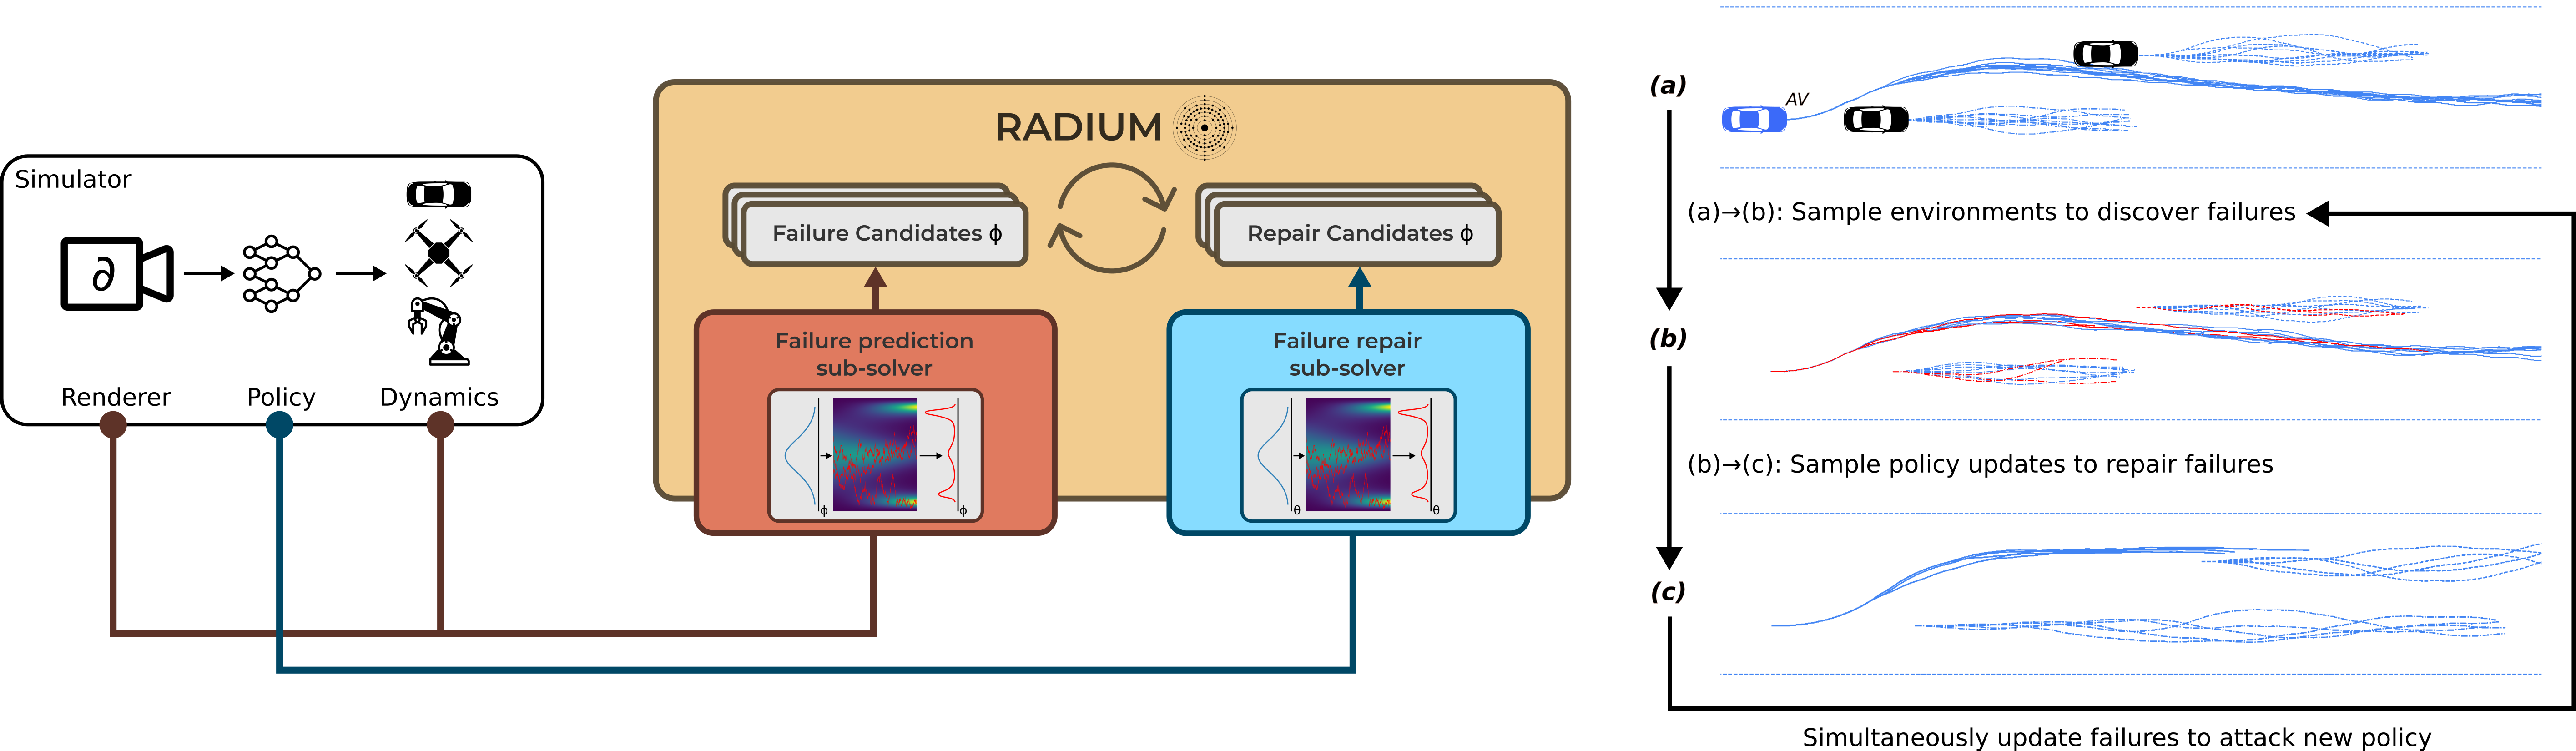
\includegraphics[width=\linewidth]{images/corl/architecture.png}
    \caption{An overview of our approach for closed-loop rare-event prediction, which efficiently predicts and repairs failures in autonomous systems. Our framework alternates between failure prediction and repair sub-solvers, which use a simulated environment to efficiently sample from the distributions~\eqref{ch:corl:eq:failure_logprob_basic} and~\eqref{ch:corl:eq:repair_logprob_basic}. We use differentiable rendering and simulation to accelerate our method with end-to-end gradients, but we also propose a gradient-free implementation.}\label{ch:corl:fig:architecture}
\end{figure}

\paragraph{Challenge 1: Distribution shift during retraining} Previous methods have proposed generating failure examples for use in retraining, but there is an inherent risk of distribution shift when doing so. Once we repair the policy, previously-predicted failures become stale and are no longer useful for verification (i.e. the distribution of likely failures has shifted). In the worst case, this can lead to overconfidence if we claim to have repaired all previously-discovered failures while remaining vulnerable to other failures. To address this issue, we interleave failure and repair steps to continuously update the set of predicted failures as we repair the policy, creating an adversarial sampling process that generates a robust repaired policy along with a set of salient failure cases.

\paragraph{Challenge 2: Exploring diverse failure modes} Traditional methods like Markov chain Monte Carlo (MCMC) are able to sample from non-normalized likelihoods like~\eqref{ch:corl:eq:failure_logprob_basic} and \eqref{ch:corl:eq:repair_logprob_basic}, but they struggle to fully explore the search space when the likelihood is highly multi-modal. To mitigate this issue, we take inspiration from the recent success of diffusion processes \cite{songScoreBasedGenerativeModeling2023,zhongGuidedConditionalDiffusion2022} and sequential Monte Carlo algorithms \cite{rubinoIntroductionRareEvent2009a} that interpolate between an easy-to-sample prior distribution and a multi-modal target distribution. Instead of sampling directly from the posterior, we begin by sampling from the unimodal, easy-to-sample prior and then smoothly interpolate to the posterior distributions~\eqref{ch:corl:eq:failure_logprob_basic}-\eqref{ch:corl:eq:repair_logprob_basic}. This process yields the tempered likelihood functions:
%
\begin{align}
    \tilde{p}_{\rm{failure}} & \propto p_{\phi, 0}(\phi)e^{-\tau[J^* - J(\theta, \phi)]_+} \label{ch:corl:eq:failure_logprob_tempered}                                     \\
    %
    \tilde{p}_{\rm{repair}}  & \propto p_{\theta, 0}(\theta, \theta_0)e^{-\frac{\tau}{n}\sum_{\phi_i}[J(\theta, \phi_i)-J^*]_+} \label{ch:corl:eq:repair_logprob_tempered}
\end{align}
%
where the tempering parameter $\tau$ is smoothly varied from $0$ to $1$. When $\tau = 0$, this is equivalent to sampling from the prior distributions, and when $\tau \to 1$ we recover the full posteriors~\eqref{ch:corl:eq:failure_logprob_basic}-\eqref{ch:corl:eq:repair_logprob_basic}. This tempering process reduces the risk of overfitting to one particular mode of the failure distribution and encourages even exploration of the failure space.

\paragraph{Challenge 3: Efficiently sampling in high dimension}
%
Previous works have proposed a wide variety of sampling algorithms that might be used as sub-solvers in our framework, including MCMC methods like random-walk Metropolis-Hastings (RMH;~\cite{hastingsMonteCarloSampling1970}), Hamiltonian Monte Carlo (HMC;~\cite{nealMCMCUsingHamiltonian2011}), and the Metropolis-adjusted Langevin algorithm (MALA;~\cite{julianbresagCommentsGrenadierMiller1994}), variational inference methods like Stein Variational Gradient Descent (SVGD;~\cite{liuSteinVariationalGradient2016a}), and other black-box methods like adaptive importance sampling~\cite{okellyScalableEndtoEndAutonomous2018}. RADIUM is able to use any of these sampling methods as sub-solvers for either the prediction or repair. Generally, these sampling methods can be classified as either gradient-free or gradient-based. Theoretical and empirical evidence suggests that gradient-based methods can enjoy faster mixing time in high dimensions on certain classes of sufficiently smooth (but non-convex) problems~\cite{maSamplingCanBe2019}, but autonomous systems with visual feedback have historically  been treated as black-boxes due to an inability to backpropagate through the rendering step \cite{zhouRoCUSRobotController2021,okellyScalableEndtoEndAutonomous2018,sinhaNeuralBridgeSampling2020}.
%
To enable the use of gradient-based samplers in RADIUM, we draw upon recent advances in differentiable simulation and rendering~\cite{huDiffTaichiDifferentiableProgramming2019,lelidecDifferentiableRenderingPerturbed2021} provide end-to-end gradients. In Sections~\ref{ch:corl:theory} and~\ref{ch:corl:experiments}, we provide theoretical and empirical evidence of a performance advantage for gradient-based samplers, but in order to make RADIUM compatible with existing non-differentiable simulators we also conduct experiments where RADIUM uses gradient-free sampling subroutines.

\subsection{RADIUM}

Pseudocode for RADIUM is provided in Algorithm~\ref{ch:corl:alg:adv_diffusion}. The algorithm maintains a population of candidate repaired policies $[\theta_1, \ldots, \theta_n]$ and failures $[\phi_1, \ldots, \phi_n]$ that are updated over $N$ sampling rounds. In each round, we sample a set of new candidate policies from the repair pseudo-posterior~\eqref{ch:corl:eq:repair_logprob_tempered}, then sample a new set of failures that attack the current population of policies. In practice, we average the tempered failure log probability~\eqref{ch:corl:eq:failure_logprob_tempered} over the population of candidate designs, which results in a smoother distribution.

RADIUM supports a wide range of subroutines for sampling candidate failures and repaired policies. In our experiments and the provided implementation, we include RMH and MALA (gradient-free and gradient-based MCMC algorithms, respectively). We choose these particular methods to provide a direct comparison between similar algorithms with and without gradients, as MALA reduces to RMH when the gradient is zero. Pseudocode for MALA is included in Algorithm~\ref{ch:corl:alg:mala}.

A final practical consideration is that although the stochasticity in our sampling-based approach can help us explore the design and failure spaces, we incur a degree of sub-optimality as a result. When using gradient-based sampling, we have the option to reduce this sub-optimality by ``quenching'' the solution: switching to simple gradient descent (e.g. using MALA for the first 90 rounds and then gradient descent on the last 10 rounds). In practice, we find that quenching can noticeably improve the final cost without compromising the diversity of predicted failure modes. Quenching is particularly important on problems where the cost function includes penalty terms for constraint satisfaction, where a few rounds of gradient descent can help to satisfy these constraints.

\begin{algorithm}
    \SetAlgoLined
    \SetKwInput{Input}{Input}
    \SetKwInput{Return}{Return}
    \Input{$N$ rounds, $K$ steps per round, stepsize $\lambda$, population size $n$, tempering rate $\alpha$, sampling algorithm (e.g. MALA as in Alg.~\ref{ch:corl:alg:mala})}

    Sample initial failures and policies using priors: $[\phi_1, \ldots, \phi_n]_0 \overset{\mathrm{iid}}{\sim} p_{\phi, 0},\ [\theta_1, \ldots, \theta_n]_0 \overset{\mathrm{iid}}{\sim} p_{\theta, 0}$\;

    \For{$i = 1, \ldots, N$}{
        $\tau \gets 1 - e^{-\alpha i / N}$\tcp*{Tempering schedule}
        %
        Sample $[\theta_1, \ldots, \theta_n]_i \overset{\mathrm{iid}}{\sim}$ \eqref{ch:corl:eq:repair_logprob_tempered}\tcp*{Sample repaired policies}\label{ch:corl:line:policy_update1}
        %
        % ${\theta_i}^* \gets \overset{\phantom{iid}}{\argmax_i} $ \eqref{ch:corl:eq:repair_logprob_tempered}\tcp*{Choose new best policy}\label{ch:corl:line:policy_update2}
        %
        Sample $[\phi_1, \ldots, \phi_n]_i \overset{\mathrm{iid}}{\sim}$ \eqref{ch:corl:eq:failure_logprob_tempered}\tcp*{Generate failures attacking $\theta^*_i$}\label{ch:corl:line:env_update}
    }

    \Return{Repaired policy $\theta^*_N = \argmax_i$ \eqref{ch:corl:eq:repair_logprob_tempered} and failures $[\phi_1, \ldots, \phi_n]_N$ attacking that policy.}

    \caption{RADIUM: Robustness via Adversarial Diversity Using MCMC}\label{ch:corl:alg:adv_diffusion}
\end{algorithm}

\subsection{Theoretical analysis}\label{ch:corl:theory}

The iterative adversarial sampling process defined in Alg.~\ref{ch:corl:alg:adv_diffusion} raises a few theoretical questions. First, when can we expect the individual sampling steps on lines~\ref{ch:corl:line:policy_update1} and~\ref{ch:corl:line:env_update} to converge, and under what conditions might we expect a gradient-based sampling sub-routine to converge faster than a gradient-free one? Second, assuming that these individual samplers converge, what sort of policies will result from the adversarial sampling loop in Alg.~\ref{ch:corl:alg:adv_diffusion}?

\paragraph{Convergence and gradient acceleration}
RADIUM inherits the asymptotic convergence guarantees of the particular subsolvers used for each sampling step. For example, when using an MCMC sampler, so long as that sampler can propose arbitrarily large steps with non-zero probability and satisfies the detailed balance condition (e.g. through the use of a Metropolis adjustment), then the sampler will produce samples asymptotically close to the target sampling distribution. Since the conditions for asymptotic convergence of MCMC samplers are relatively weak~\cite{hastingsMonteCarloSampling1970}, it is more interesting to ask about finite-sample convergence rates; in particular, under what conditions can we expect gradient-based samplers like MALA to accelerate convergence to the target distribution?

In many robotics problems, even when analytical gradients are available, it is unclear whether these gradients are useful for optimization (i.e. low empirical bias and variance;~\cite{suhDifferentiableSimulatorsGive2022}). Here, we build on recent theoretical results by~\cite{maSamplingCanBe2019} to provide sufficient conditions for fast, polynomial-time convergence of gradient-based samplers in our setting. With slight abuse of notation, we use $J(\theta, \phi)$ to denote the composition of the simulator and cost function.

\begin{theorem}\label{ch:corl:thm:convergence}
    Let $J(\theta, \phi)$ be a $L$-Lipschitz smooth cost function (i.e. $\nabla J$ is $L$-Lipschitz continuous), let the log prior distributions $\log p_{\phi ,0}$ and $\log p_{\theta,0}$ be Lipschitz smooth everywhere and $m$-strongly convex outside a ball of finite radius $R$, and let $d = \max\pn{\dim{\theta}, \dim{\phi}}$ be the dimension of the search space. If $m > L$, then MALA with appropriate step size will yield samples within $\epsilon$ total variation distance of the target distributions~\eqref{ch:corl:eq:failure_logprob_tempered} and~\eqref{ch:corl:eq:repair_logprob_tempered} with total number of sampling steps $\leq \widetilde{\mathcal{O}}\pn{d^2 \ln\frac{1}{\epsilon}}$.
\end{theorem}

The key idea of the proof is to rely on the log-concavity of the prior distributions to dominate the non-convexity of the cost function sufficiently far from the central modes.

\begin{proof}
    We will show the proof for sampling from the failure generating process with likelihood given by Eq.~\eqref{ch:corl:eq:failure_logprob_tempered}; the proof for the repair generating process follows similarly. The log-likelihood for the failure generating process is
    \begin{equation}
        \log p_{\phi, 0}(\phi) - \tau [J^* - J(\theta, \phi)]_+ \label{ch:corl:eq:failure_logprob}
    \end{equation}

    \cite{maSamplingCanBe2019} show that MALA sampling enjoys the convergence guarantees of Theorem~\ref{ch:corl:thm:convergence} so long as the target log likelihood is strongly convex outside of a ball of finite radius $R$ (see Theorem 1 in \cite{maSamplingCanBe2019}). Since $\log p_{\phi, 0}(\phi)$ is assumed to be strongly $m$-convex, it is sufficient to show that as $||\phi|| \to \infty$, the strong convexity of the log-prior dominates the non-convexity in $\tau [J^* - J(\theta, \phi)]_+$.

    For convenience, denote $f(\phi) = -\tau [J^* - J(\theta, \phi)]_+$ and $g(\phi) = \log p_{\phi, 0}(\phi)$. We must first show that $f(\phi) + g(\phi)$ is $(m-L)$-strongly convex, for which it suffices to show that $f(\phi) + g(\phi) - (m-L)/2 ||\phi||^2$ is convex. Note that
    \begin{align}
        f(\phi) + g(\phi) - \frac{m-L}{2} ||\phi||^2 & = f(\phi) + \frac{L}{2} ||\phi||^2 + g(\phi) - \frac{m}{2} ||\phi||^2
    \end{align}
    $g(\phi) - \frac{m}{2} ||\phi||^2$ is convex by $m$-stong convexity of $g$, so we must show that the remaining term, $f(\phi) + L/2 ||\phi||^2$, is convex. Note that the Hessian of this term is $\nabla^2 f(\phi) + LI$. Since we have assumed that $J$ is $L$-Lipschitz smooth (i.e. its gradients are $L$-Lipschitz continuous), it follows that the magnitudes of the eigenvalues of $\nabla^2 f$ are bounded by $L$, which is sufficient for $\nabla^2 f(\phi) + LI$ to be positive semi-definite, completing the proof.
\end{proof}

Theorem~\ref{ch:corl:thm:convergence} requires smoothness assumptions on the cost; we recognize that this assumption is difficult to verify in practice and does not hold in certain domains (notably when rigid body contact is involved). However, in the problems we consider it is possible to smooth the simulator (e.g. using smoothed dynamics and a blurred renderer and scene representation), thus smoothing the gradients of $J$. The smoothness and convexity conditions hold for many common prior distributions, such as Gaussian and smoothed uniform distributions.

\paragraph{Adversarial Joint Distribution} Even if the samplers for both policy and environmental parameters converge within each round of Alg.~\ref{ch:corl:alg:adv_diffusion}, it is not clear what will be the effect of running these samplers repeatedly in an adversarial manner. Our next theoretical result defines the joint distribution of $\theta$ and $\phi$ as a result of this adversarial sampling loop. To simplify the theoretical analysis, we consider the case when population size $n=1$, and we replace the smooth ELU with a ReLU in~\eqref{ch:corl:eq:failure_logprob_basic} and~\eqref{ch:corl:eq:repair_logprob_basic}.

\begin{theorem}\label{ch:corl:thm:joint}
    The iterative adversarial sampling procedure in Alg.~\ref{ch:corl:alg:adv_diffusion} yields policies drawn from a marginal distribution with density function
    \begin{equation}
        f_\theta(\theta^*) = p_{\theta, 0}(\theta^*) \pn{\frac{\expectation_{\phi \sim p_{\phi, 0}}\left[ e^{J(\theta^*, \phi) - J^*} | J(\theta^*, \phi) \leq J^* \right]}{\expectation_{\phi \sim p_{\phi, 0}}\left[ e^{J(\theta^*, \phi) - J^*} \right]} +
            %
            \frac{\mathbb{P}[J(\theta^*, \phi) > J^*]}{\expectation_{\phi \sim p_{\phi, 0}}\left[ e^{J(\theta^*, \phi) - J^*}\right]}}\label{ch:corl:eq:marginal}
    \end{equation}
    where $\mathbb{P}(J(\theta^*, \phi) > J^* = \expectation_{\phi \sim p_{\phi, 0}}[\mathbbm{1}(J(\theta^*, \phi) \geq J^*)]$ is the probability of failure when $\phi$ is sampled from the prior distribution.
\end{theorem}

The first term in the parenthesis in~\eqref{ch:corl:eq:marginal} is bounded above by $1$ and maximized when the policy does not experience failure (in which case the conditional and unconditional expectations will be equal). The numerator of the second term bounded $[0, 1]$, while the denominator grows exponentially large when a failure occurs. As a result, the marginal distribution of $\theta^*$ assigns higher probability (relative to the prior) for policies that avoid failure.

\begin{proof}
    We can treat Alg.~\ref{ch:corl:alg:adv_diffusion} as a two-stage Gibbs sampling procedure and apply the Hammersley-Clifford Theorem~\cite{robertMonteCarloStatistical2004} to get the joint distribution
    \begin{equation}
        f_{\theta, \phi}(\theta^*, \phi^*) = p_{\theta, 0}(\theta^*) p_{\phi, 0}(\phi^*) \frac{e^{-[J^* - J(\theta^*, \phi^*)]_+}}{\expectation_{\phi \sim p_{\phi, 0}}\left[ e^{J(\theta^*, \phi) - J^*} \right]} \label{ch:corl:eq:joint}
    \end{equation}

    Integrating over $\phi$ yields the marginal distribution of $\theta$, completing the proof.
    \begin{align}
        f_{\theta^*} & = \int_\phi f_{\theta, \phi}(\theta^*, \phi) d\phi = \frac{p_{\theta, 0}(\theta^*)}{\expectation_{\phi \sim p_{\phi, 0}}\left[ e^{J(\theta^*, \phi) - J^*} \right]}  \int_\phi p_{\phi, 0}(\phi) e^{-[J^* - J(\theta^*, \phi^*)]_+} d\phi                                                                               \\
        %
                     & = p_{\theta, 0}(\theta^*)\frac{\expectation_{\phi \sim p_{\phi, 0}}\left[ e^{-[J^* - J(\theta^*, \phi)]_+} \right]}{\expectation_{\phi \sim p_{\phi, 0}}\left[ e^{J(\theta^*, \phi) - J^*} \right]}                                                                                                                     \\
        %
                     & = p_{\theta, 0}(\theta^*)\frac{\expectation_{\phi \sim p_{\phi, 0}}\left[ e^{-(J^* - J(\theta^*, \phi))} | J^* - J(\theta^*, \phi) \geq 0 \right] + \expectation_{\phi \sim p_{\phi, 0}}\left[ 1 | J^* - J(\theta^*, \phi) < 0 \right]}{\expectation_{\phi \sim p_{\phi, 0}}\left[ e^{J(\theta^*, \phi) - J^*} \right]} \\
        %
                     & = p_{\theta, 0}(\theta^*)\frac{\expectation_{\phi \sim p_{\phi, 0}}\left[ e^{-(J^* - J(\theta^*, \phi))} | J^* \geq J(\theta^*, \phi) \right] + \expectation_{\phi \sim p_{\phi, 0}}\left[ 1 | J^* < J(\theta^*, \phi) \right]}{\expectation_{\phi \sim p_{\phi, 0}}\left[ e^{J(\theta^*, \phi) - J^*} \right]}         \\
                     & = p_{\theta, 0}(\theta^*)\frac{\expectation_{\phi \sim p_{\phi, 0}}\left[ e^{-(J^* - J(\theta^*, \phi))} | J^* \geq J(\theta^*, \phi) \right] + \mathbb{P}[J(\theta^*, \phi) > J^*]}{\expectation_{\phi \sim p_{\phi, 0}}\left[ e^{J(\theta^*, \phi) - J^*} \right]}                                                    \\
    \end{align}
\end{proof}

\section{Simulation experiments}\label{ch:corl:experiments}

In this section, we provide empirical comparisons of RADIUM with existing methods for adversarial optimization and policy repair in a range of simulated environments. We have two main goals in this section. First, we seek to understand whether re-framing the failure repair problem from optimization to inference leads to better solutions (i.e. more robust designs and better coverage by the predicted failures). Second, we study whether the gradient-based version of our method yields any benefits over the gradient-free version. After the empirical comparisons in this section, Section~\ref{ch:corl:case_studies} then provides three case studies with a more in-depth discussion of how RADIUM can be applied to practical verification and design problems, including two case studies demonstrating how repaired designs can be transferred from simulation to hardware.

We conduct simulation studies on a range of problems from the robotics and cyberphysical systems literature, comparing against previously-published adversarial optimization methods. More detail on each benchmark, baseline, and implementation is provided in the appendix.

\subsection{Experimental setup}

\subsubsection{Baselines}

We compare with three baselines taken from the adversarial optimization and testing literature.
%
\textit{Gradient descent with randomized counterexamples (\gdr)} optimizes the design using a fixed set of random counterexamples, representing a generic policy optimization with domain randomization approach.
%
\textit{Gradient descent with adversarial counterexamples (\gda)} alternates between optimizing the design and optimizing for maximally adversarial failure modes, as in~\cite{hanselmannKINGGeneratingSafetyCritical2022a,dawsonRobustCounterexampleguidedOptimization2022b}.
%
\textit{Learning to collide (\ltc)} uses black-box optimization (REINFORCE) to search for failure cases~\cite{dingLearningCollideAdaptive2020a}.
%
We denote the gradient-free and gradient-based variants of RADIUM as $R_0$ and $R_1$, respectively.
%
All methods were run on the same GPU model with the same sample budget for each task. Hyperparameters for all experiments are given in the appendix.

\subsubsection{Benchmark problems}

We rely on two classes of benchmark problem in this work: 3 problems without vision in the loop, and 3 problems with vision in the loop. Each of these problem domains includes multiple environments of varying complexity, for a total of 13 different environments. A summary of these environments is given in Fig~\ref{ch:corl:fig:environments}. More details on the parameters and cost functions used for each environment are given in the supplementary material.

\begin{figure*}[t]
    \centering
    \includegraphics[width=\linewidth]{example-image-a}  % Todo
    \caption{The different environments used in our simulation studies, including 5 domains without visual feedback and 3 domains with vision in the loop.}\label{ch:corl:fig:environments}
\end{figure*}

\paragraph{Non-vision benchmarks}
%
\textit{Search:} a set of seeker robots must cover a region to detect a set of hiders. $\theta$ and $\phi$ define trajectories for the seekers and hiders, respectively. Failure occurs if any hider escapes detection by the seekers (which have fixed sensing radius). This environment has two variants: small (6 seeker vs. 10 hider, $\dim{\theta} = 60$, $\dim{\phi} = 100$) and large (12 seeker vs. 20 hider, $\dim{\theta} = 120$, $\dim{\phi} = 200$).
%
\textit{Formation control:} a swarm of drones fly to a goal while maintaining full connectivity with a limited communication radius. $\theta$ defines trajectories for each robot in the swarm, while $\phi$ defines an uncertain wind velocity field. Failure occurs when the second eigenvalue of the graph Laplacian is close to zero. This environment has small (5 agent, $\dim{\theta} = 30$, $\dim{\phi} = 1280$) and large (10 agent, $\dim{\theta} = 100$, $\dim{\phi} = 1280$) variants.
%
\textit{Power grid dispatch:} electric generators must be scheduled to ensure that the network satisfies voltage and maximum power constraints in the event of transmission line outages. $\theta$ specifies generator setpoints and $\phi$ specifies line admittances; failures occur when any of the voltage or power constraints are violated. This environment has small (14-bus, $\dim{\theta} = 32$, $\dim{\phi} = 20$) and large (57-bus, $\dim{\theta} = 98$, $\dim{\phi} = 80$) versions.
% %
% \textit{GCAS:} a ground collision avoidance system (GCAS) must be designed to prevent a jet aircraft, modeled with aerodynamic effects and engine dynamics, from crashing into the ground. $\theta$ defines a control policy neural network ($\dim{\theta}\approx 1.8\times10^3$) and $\phi$ defines the initial conditions ($\dim{\phi} = 5$).
% %
% \textit{Pushing:} a robot manipulator must push an object out of the way to reach another object. Failure occurs if the object is knocked over while pushing. $\theta$ defines a planning policy network ($\dim{\theta} \approx 1.2\times10^3$) and $\phi$ defines the unknown inertial and frictional properties of the object being pushed, as well as measurement noises ($\dim{\phi} = 7$).

\paragraph{Vision-in-the-loop benchmarks}

\textit{AV (highway):} An autonomous vehicle must overtake two other vehicles.
%
\textit{AV (intersection):} the autonomous vehicle must navigate an uncontrolled intersection with crossing traffic.
%
In both AV tasks, the actions of the non-ego vehicles are uncertain, and the AV observes RGBd images from a front-facing camera as well as its own speed.
%
\textit{Drone:} A drone must safely navigate through a cluttered environment in windy conditions. There is uncertainty in the wind speed and location of all obstacles.
%  \textit{Drone (dynamic):} the same but the obstacles move with uncertain velocities.
%
Initial convolutional neural network (CNN) policies $\theta_0$ for drone and intersection environments were pretrained using behavior cloning, and CNN-based policies for the highway environment were pretrained using PPO~\cite{schulmanProximalPolicyOptimization2017}.
%
\textit{Grasp (box/mug): } a robot must locate and grasp an object using a depth image of the scene. There is uncertainty in the location of the objects and in the location of a nearby distractor object. The grasp detector is trained with labels of ground-truth grasp affordances.

The dimension of the failure space is 20 for the highway task, 30 for the intersection task, 12 for the drone task, and 4 for the grasping tasks. The dimension of the policy space is 64k for the highway and intersection tasks, 84k for the drone task, and 266k for the grasping tasks.

\subsubsection{Implementation}

Since we require a differentiable renderer and simulation engine for our work, we were not able to use an off-the-shelf simulator like CARLA~\cite{Dosovitskiy17}. Instead, we write our own simulator and basic differentiable renderer using JAX, which is available at \url{github.com/MIT-REALM/architect_corl_23}.
%
Likewise, our method and all baselines were implemented in JAX and compiled using JAX's just-in-time (JIT) compilation. Each metric reports the mean and standard deviation across four independent random seeds. All methods are given the same total sample budget for both prediction and repair (except for \gdr, which does not update the predicted failure modes).

The non-vision benchmarks were all initialized with random $\theta_0$, and the vision benchmarks were initialized using $\theta_0$ trained using reinforcement learning or behavior cloning with domain randomization. We include comparisons with \gdr, \gda, and \ltc{} on all non-vision benchmarks. Since $\theta_0$ on the vision benchmarks was trained using domain randomization, \gdr{} is not able to improve the initial parameters, and so we include comparisons with $\theta_0$, \gda, and \ltc{} for the vision benchmarks.

\subsubsection{Metrics}

To measure the robustness of the optimized policies, we report the failure rate (FR) on a test set of 1,000 i.i.d. samples of $\phi$ from the prior $p_{\phi, 0}$. We also report the mean cost on this test set as well as the maximum cost on the vision-in-the-loop benchmarks (where cost is bounded by construction) and the 99\textsuperscript{th}-percentile cost for non-vision benchmarks (some of which have unbounded cost, making the 99\textsuperscript{th} percentile more representative). Costs are normalized by the maximum cost observed across any method. Finally, for each task, we report the time required to run a simulation both with and without reverse-mode differentiation.

\subsection{Results}

Fig.~\ref{ch:corl:fig:nonvision_results} shows the results from benchmark problems without vision in the loop, while Fig.~\ref{ch:corl:fig:vision_results} shows the results from problems with vision in the loop. For ease of comparison, each plot groups the gradient-free methods (\ltc{} and $R_0$) and the gradient-based methods (\gdr, \gda, and $R_1$). Since the initial parameters for the vision-in-the-loop benchmarks in Fig.~\ref{ch:corl:fig:vision_results} were trained using RL or behavior cloning (which do not require differentiable simulation), we group $\theta_0$ with the gradient-free results in Fig.~\ref{ch:corl:fig:vision_results}. We also compare the convergence rates of each method in Fig.~\ref{ch:corl:fig:convergence}. Table~\ref{ch:corl:tab:runtime} shows the time required for simulating with and without automatic differentiation.

\begin{figure}[tb]
    \centering
    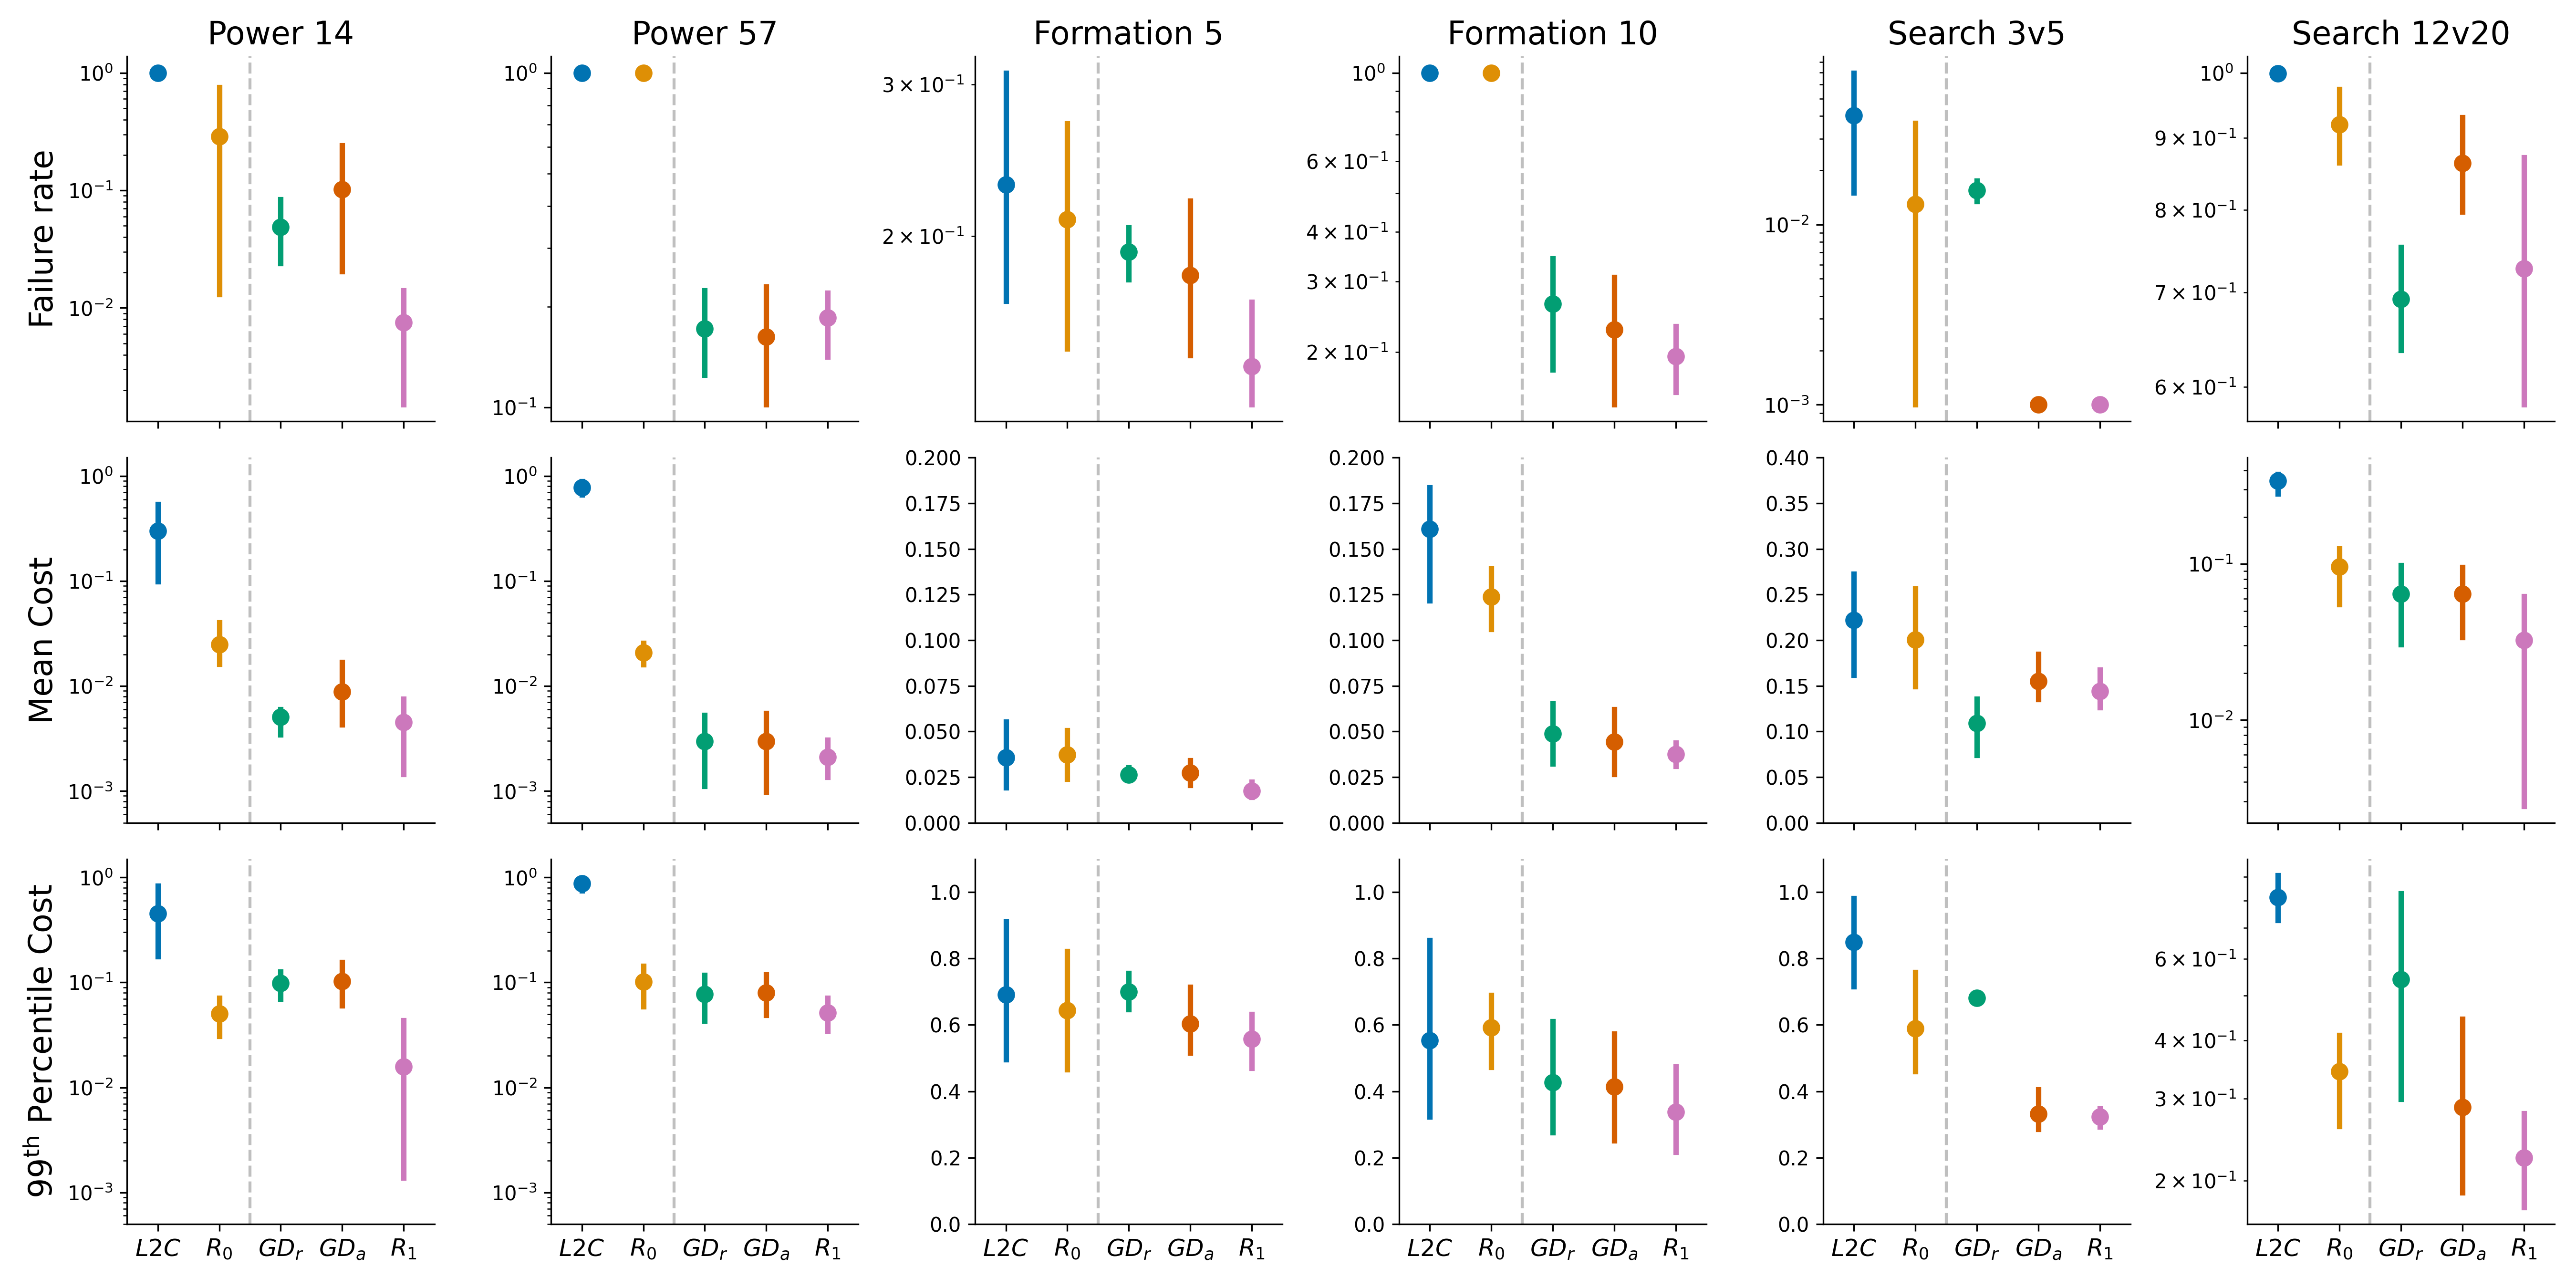
\includegraphics[width=\linewidth]{images/corl/nonvision.png}
    \caption{Comparison of our method (gradient-free and gradient-based variants $R_0$ and $R_1$, respectively) and baseline methods on benchmark problems without vision in the loop, showing failure rate, mean cost, and 99\textsuperscript{th} percentile cost on a test set of 1,000 randomly sampled $\phi$. The dashed gray lines separate gradient-free and gradient-based methods.}\label{ch:corl:fig:nonvision_results}
\end{figure}

\begin{figure}[tb]
    \centering
    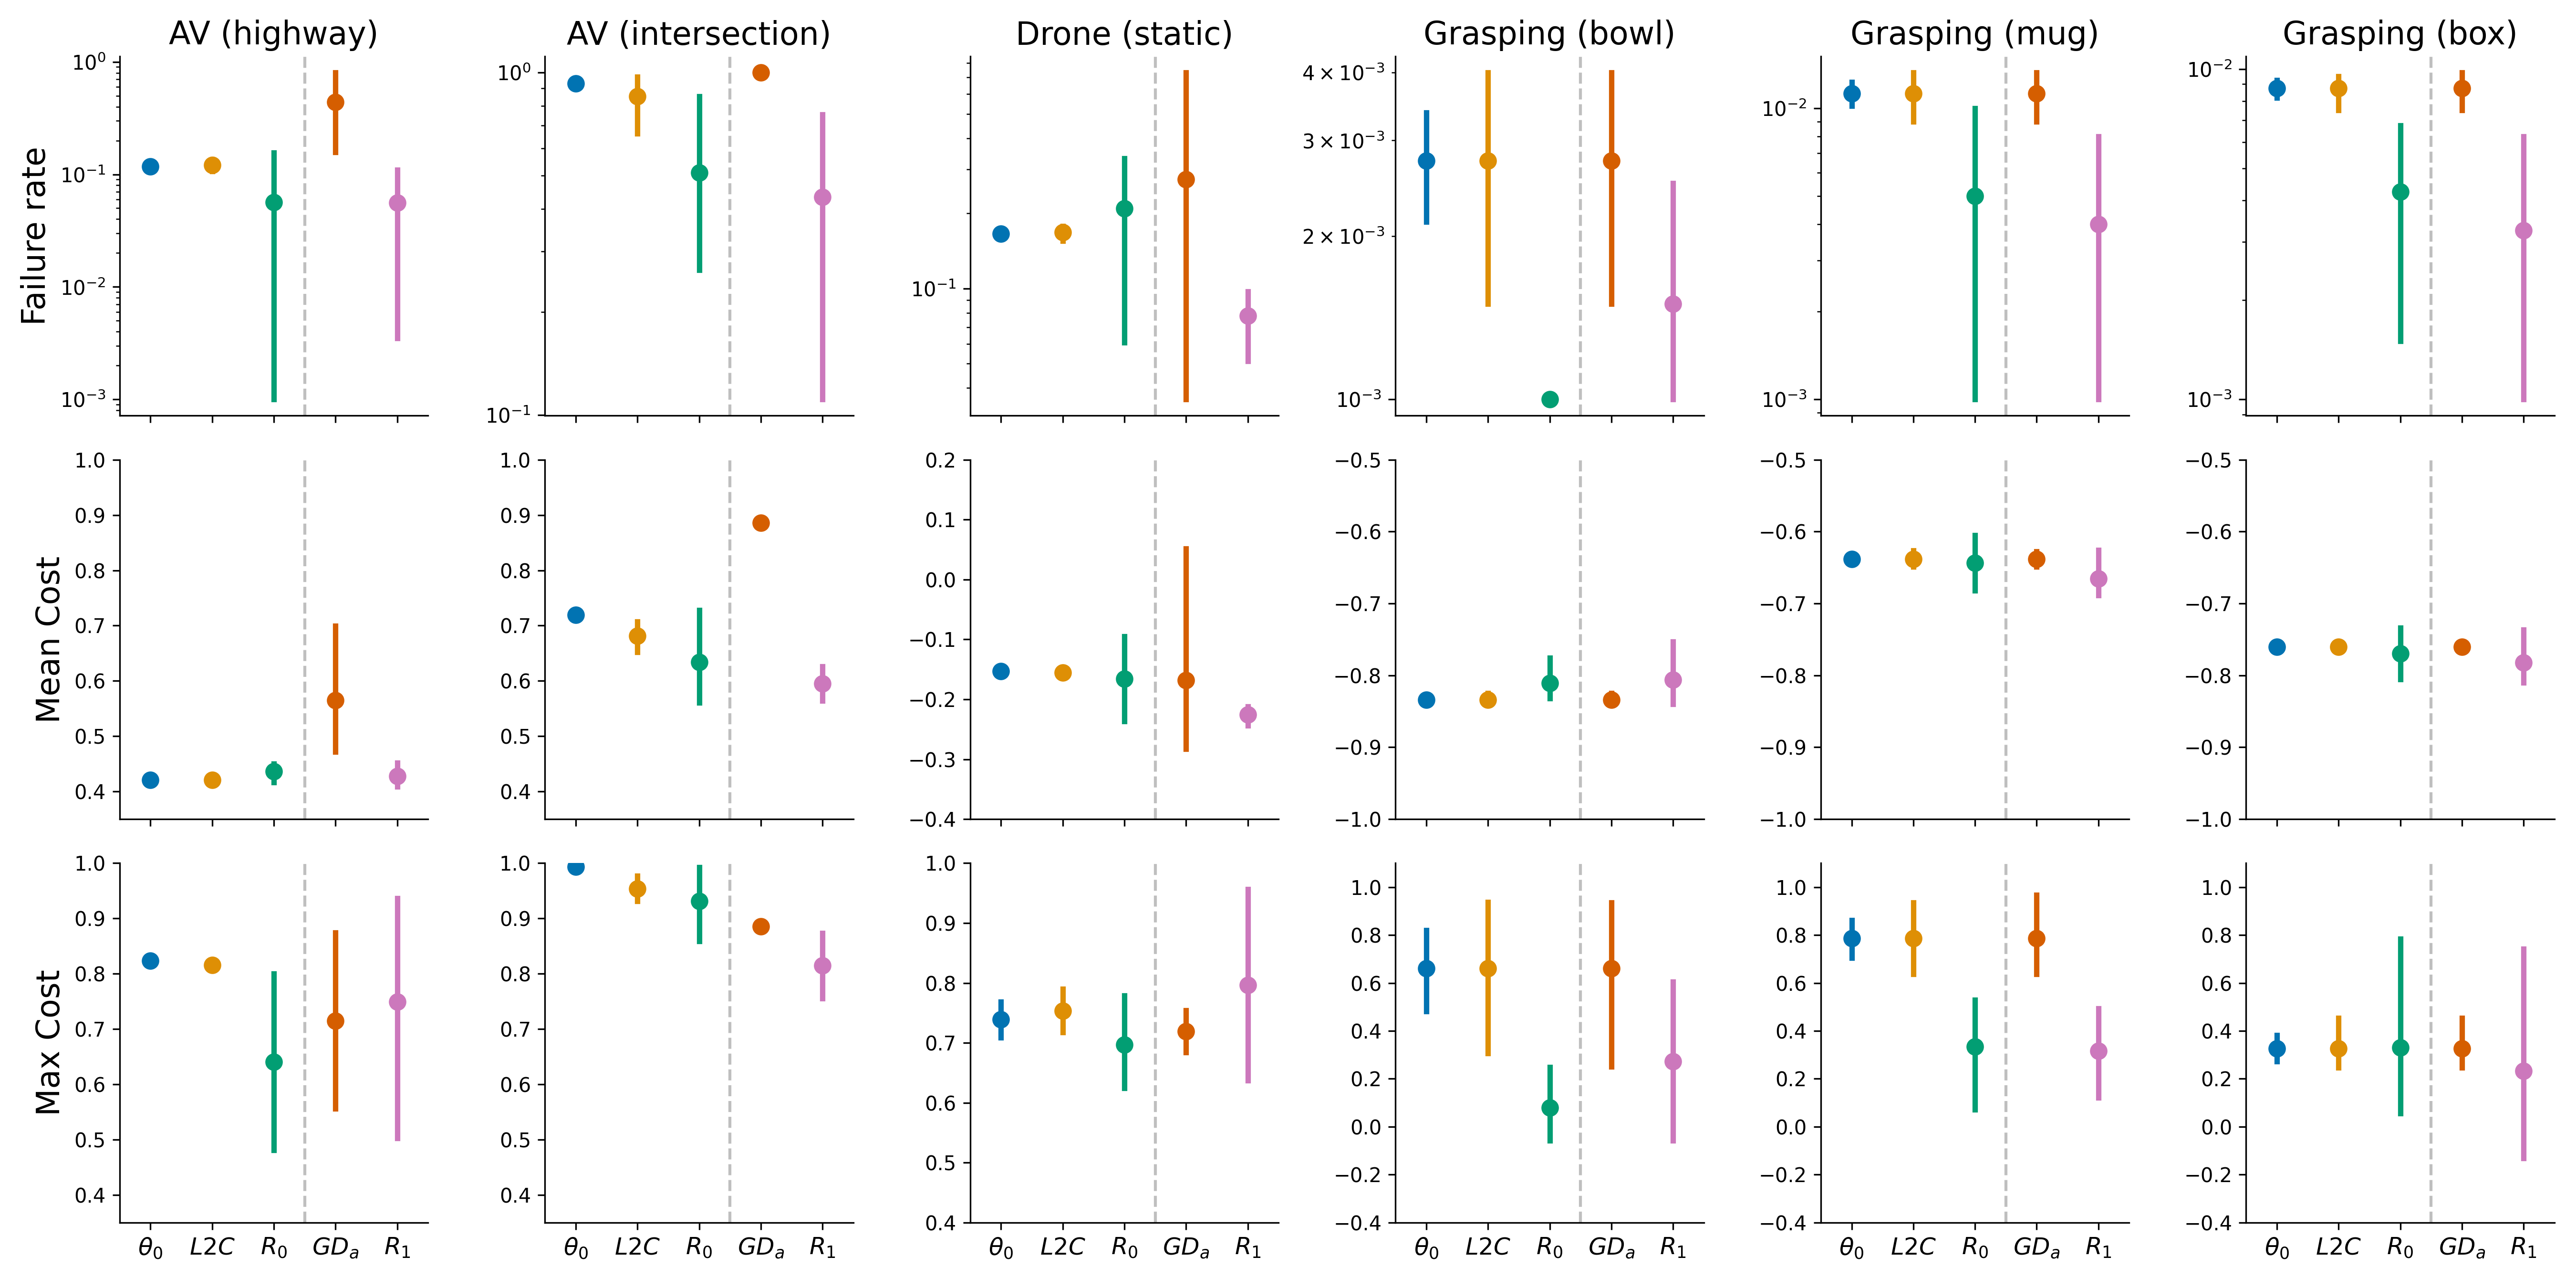
\includegraphics[width=\linewidth]{images/corl/vision.png}
    \caption{Comparison of our method (gradient-free and gradient-based variants $R_0$ and $R_1$, respectively) and baseline methods on benchmark problems with vision in the loop, showing failure rate, mean cost, and max cost on a test set of 1,000 randomly sampled $\phi$. The dashed gray lines separate gradient-free and gradient-based methods.}\label{ch:corl:fig:vision_results}
\end{figure}

\begin{figure}[tb]
    \centering
    \begin{subfigure}[t]{\linewidth}
        \centering
        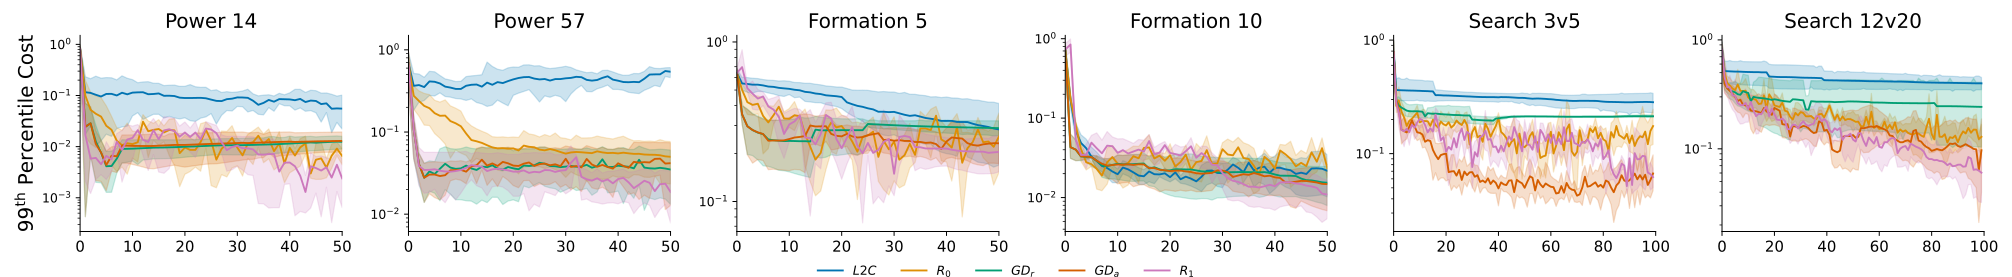
\includegraphics[width=\linewidth]{images/corl/nonvision_convergence.png}
        \caption{Non-vision benchmarks}\label{ch:corl:fig:convergence:nonvision}
    \end{subfigure}
    \begin{subfigure}[t]{\linewidth}
        \centering
        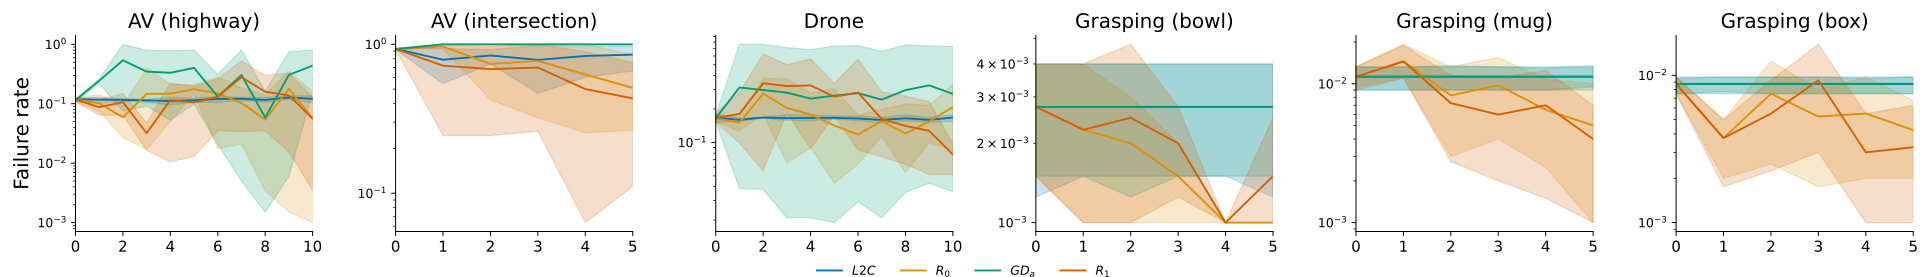
\includegraphics[width=\linewidth]{images/corl/vision_convergence.png}
        \caption{Vision-in-the-loop benchmarks}\label{ch:corl:fig:convergence:vision}
    \end{subfigure}
    \caption{Convergence rates of our method and baselines on tasks with (top) and without (bottom) vision in the loop.}\label{ch:corl:fig:convergence}
\end{figure}

Fig.~\ref{ch:corl:fig:repairs} shows examples of failure cases and repaired policies generated using $R_1$ on three vision-in-the-loop tasks: AV (highway), AV (intersection), and drone. The left of Fig.~\ref{ch:corl:fig:repairs} shows the initial policy $\theta_0$ and failure modes discovered using our method (sampling $\phi$ while holding $\theta_0$ fixed), while the right shows the repaired policy and updated challenging counterexamples. Since the distribution of failure modes shifts as we repair the policy, we continuously re-sample the failure modes to be relevant to the updated policy. In all cases, we see that the repaired policy found using our method experiences fewer failures, despite the updated adversarial failure modes. In certain cases, the repaired policy exhibits a qualitatively different behavior; for example, in the vision-in-the-loop highway control task, the repaired policy is less aggressive than the original policy, avoiding the risky overtake maneuver (top row of Fig.~\ref{ch:corl:fig:repairs}).

\begin{figure}[t]
    \centering
    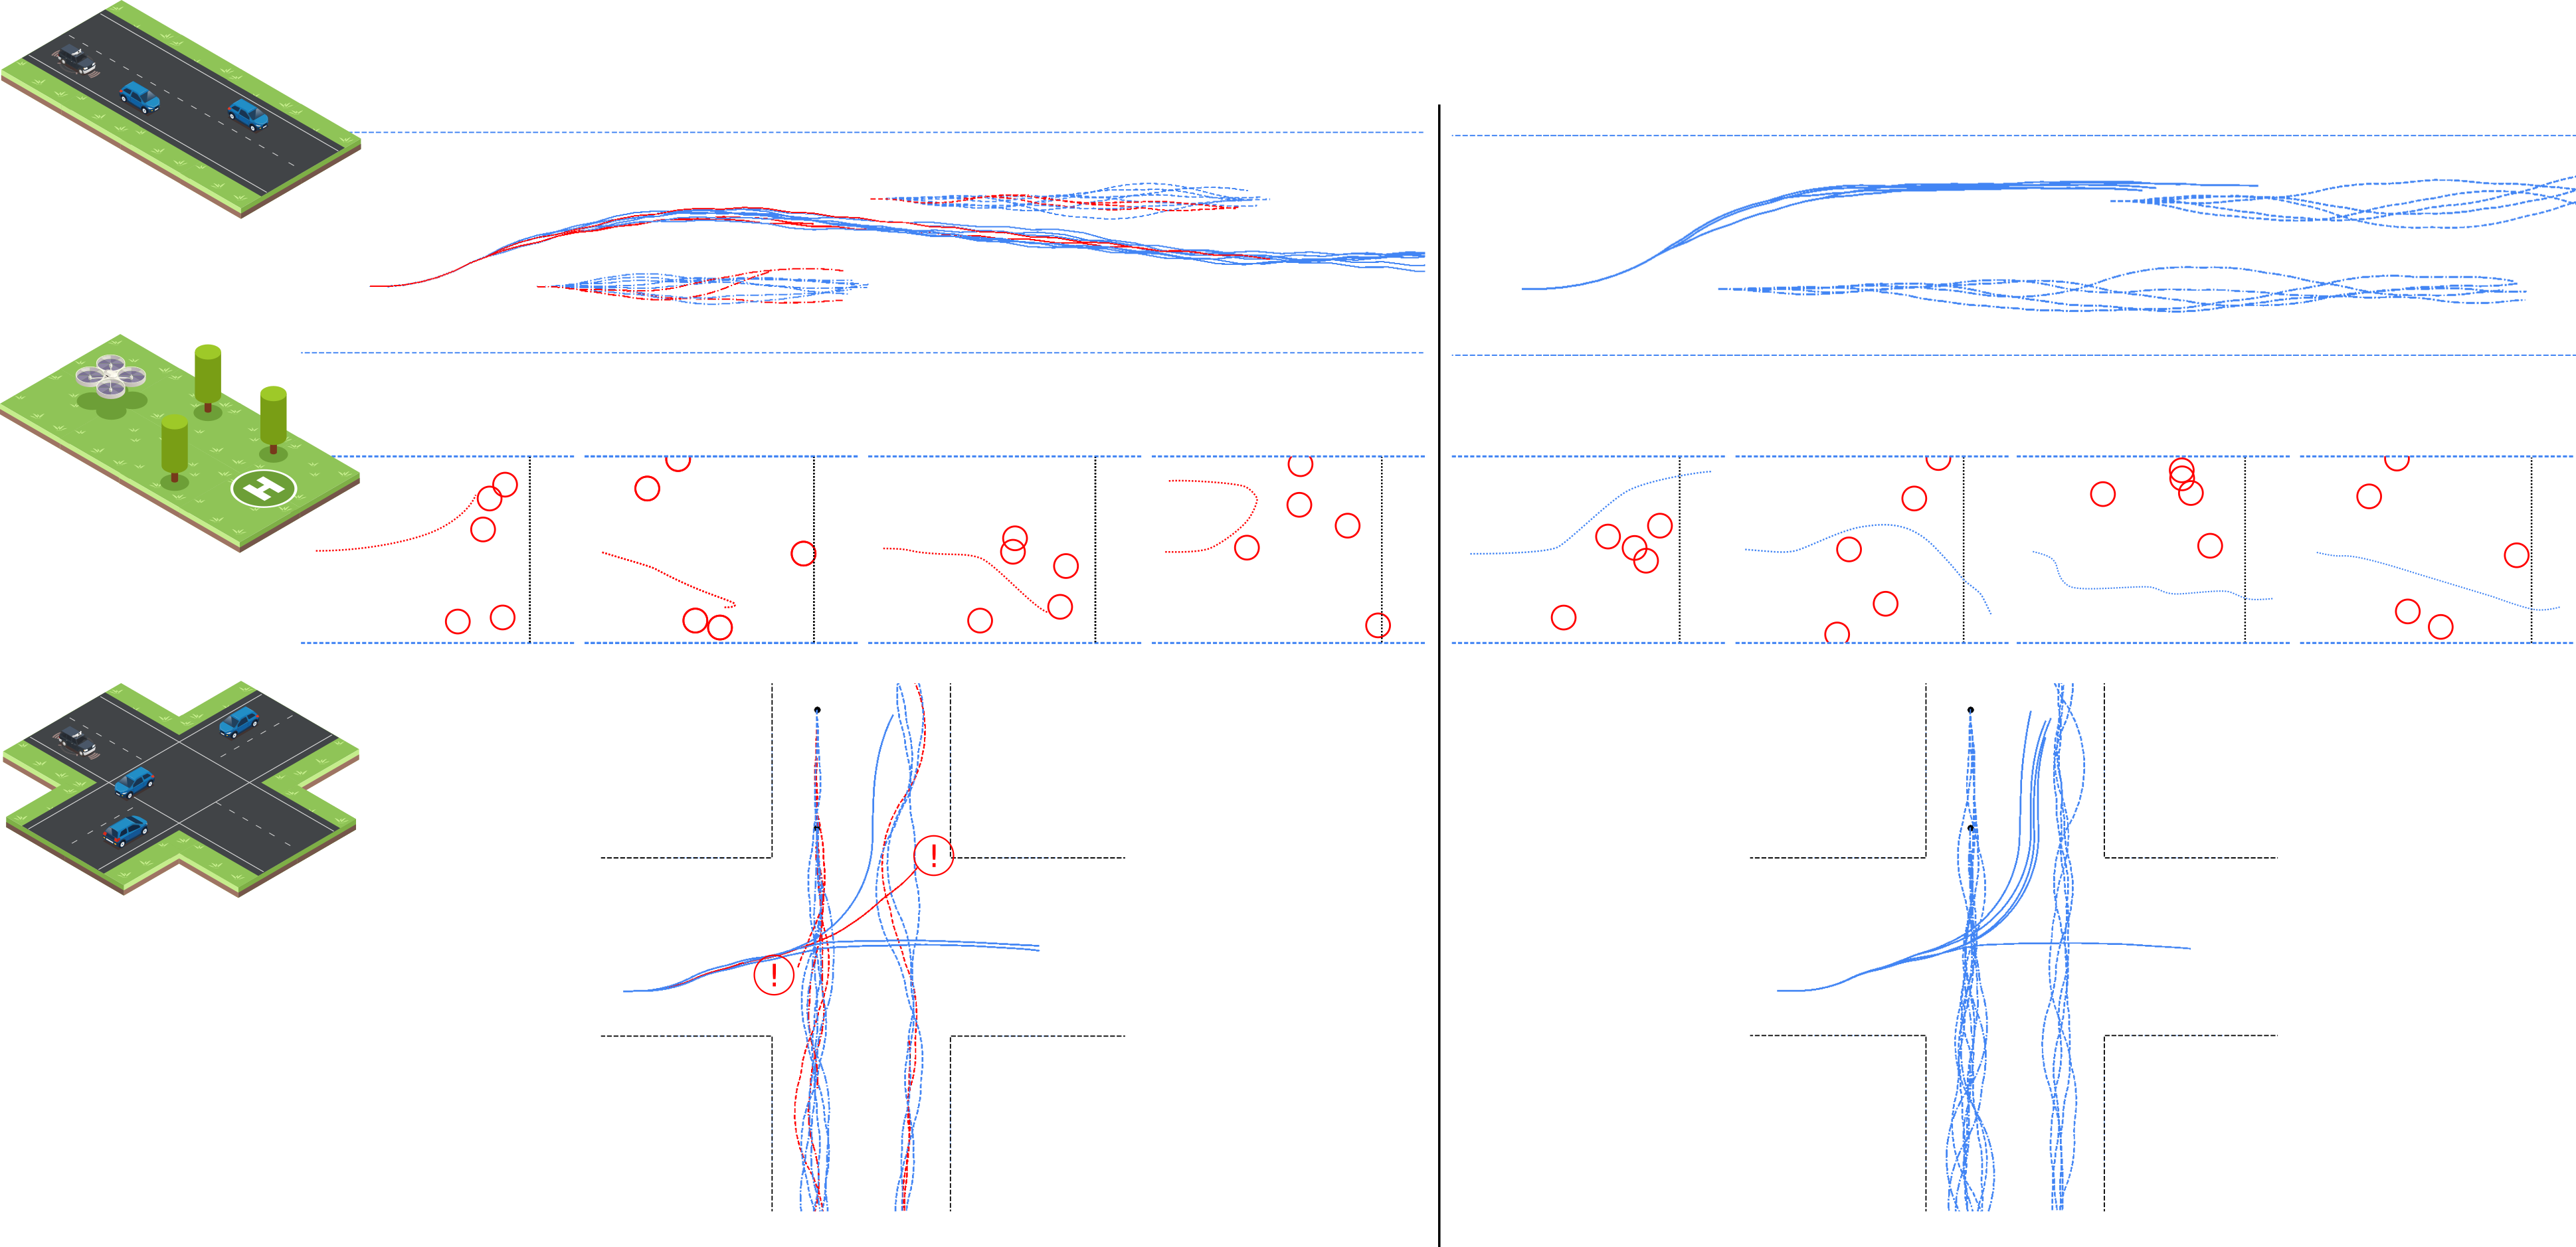
\includegraphics[width=\linewidth]{images/corl/repairs.png}
    \caption{Examples of failure cases (left) and repaired policies (right) generated using our method. Failed trajectories are shown in red.}\label{ch:corl:fig:repairs}
\end{figure}

\begin{table}
    \caption{Time required for simulating a rollout with and without autodiff (AD) for each task (in seconds). Average and standard deviation (subscript) reported across 100 trials on AMD Ryzen Threadripper 3990X 64-Core Processor (non-vision tasks) and an NVIDIA RTX A4000 (vision-in-the-loop tasks).}
    \label{ch:corl:tab:runtime}
    \centering
    \scriptsize
    \begin{tabular}{rcccccc}
        \toprule
        \multicolumn{1}{l}{} & \multicolumn{6}{c}{Non-vision tasks}                                                                                                                       \\
        \cmidrule(r){2-7}
                             & Power (14)                             & Power (57)         & Formation (5)     & Formation (10)               & Search (3v5)        & Search (12v20)      \\
        \midrule
        w/o AD               & $0.00122_{0.00413}$                    & $0.0107_{0.00893}$ & $0.0326_{0.0173}$ & $0.628_{0.296}$              & $0.00147_{0.00461}$ & $0.00461_{0.00747}$ \\
        w/ AD                & $0.00165_{0.00488}$                    & $0.0136_{0.0111}$  & $0.0543_{0.0212}$ & $0.714_{0.306}$              & $0.00358_{0.00704}$ & $0.0107_{0.00851}$  \\
        \midrule
        \multicolumn{1}{l}{} & \multicolumn{6}{c}{Vision-in-the-loop}                                                                                                                     \\
        \cmidrule(r){2-7}
                             & AV (hw.)                               & AV (int.)          & Drone             & Grasp (all)                  &                     &                     \\
        \midrule
        w/o AD               & $0.70_{0.003}$                         & $2.22_{0.01}$      & $0.39_{0.002}$    & $0.0045_{5.1\times 10^{-5}}$ &                                           \\
        w/ AD                & $1.72_{0.003}$                         & $6.65_{0.14}$      & $1.77_{0.06}$     & $0.0049_{3.8\times 10^{-5}}$ &                                           \\
        \bottomrule
    \end{tabular}
\end{table}

\subsection{Discussion}

In our results on problems without vision in the loop (Fig.~\ref{ch:corl:fig:nonvision_results}), we see several high-level trends. First, we see that gradient-based techniques (\gdr, \gda, and $R_1$) achieve lower failure rates, mean cost, and 99\textsuperscript{th} percentile costs relative to gradient-free methods (\ltc{} and $R_0$) on the test set, likely because gradient information helps the former methods explore the high-dimensional search space (as seen in the faster convergence of gradient-based methods in Fig.~\ref{ch:corl:fig:convergence:nonvision}). Moreover, we find that our methods ($R_0$ and $R_1$) outperform other methods within each of their respective categories; i.e. $R_0$ yields repaired solutions with lower costs and failure rates than \ltc, and $R_1$ likewise outperforms \gdr{} and \gda{}.

We see a slightly different pattern in our results for problems with vision in the loop. On these problems, we find that existing gradient-based methods like \gda{} do not achieve lower failure rates than gradient-free methods like \ltc{}, possibly due to poor gradient quality from the differentiable renderer (where occlusions can lead to large variance in the automatically-derived gradients). In contrast, both variants of our method achieve low failure rates for repaired policies in the vision-in-the-loop tasks, and $R_1$ in particular is able to achieve better performance on some tasks because the Metropolis-Hastings adjustment on line~\ref{ch:corl:alg:mala:mh} of Algorithm~\ref{ch:corl:alg:mala} allows it to reject large steps caused by poorly conditioned gradients.

\section{Case studies}\label{ch:corl:case_studies}

In this next section, we present three case studies to illustrate the practical use of our method. We first demonstrate how RADIUM can be used to solve a challenging optimization problem arising in the control of electrical power systems. We then provide two case studies showing how RADIUM can be applied to robotics problems and transferred to hardware.  %  TODO one case study for draft for committee

\subsection{Robust generation dispatch for secure power networks}

For our first case study, we consider the problem of controlling an electric power grid subject to failures in transmission lines. Two simple networks (the IEEE 14- and 57-node test system) are shown in Fig.~\ref{ch:corl:fig:networks}. The goal in this problem is to find control inputs (power injection and voltage at each generator, and power demand at each load) that ensure that the voltage seen by each load is stable, even in the event of transmission outages (which we model using a bimodal distribution for the admittance of each line). The simulator models the AC power flow through this network, and the cost function penalizes excessively high or low voltages or any violation of rated generator capacities. More details on this motivating example is provided in the appendix.

Given a transmission network, the so-called \textit{security-constrained optimal power flow problem} (or SCOPF~\cite{capitanescuStateoftheartChallengesFuture2011}) is the problem of scheduling generator setpoints and power demand from loads to minimize the economic cost of generation and ensure that the network operates safely (satisfying voltage and maximum power constraints) in the event of transmission line outages. The design parameters $x = (P_g, |V|_g, P_l, Q_l)$ include the real power injection $P_g$ and AC voltage amplitude $|V|_g$ at each generator in the network and the real and reactive power draws at each load $P_l, Q_l$; all of these parameters are subject to minimum and maximum bounds that we model using a uniform prior distribution $p_{x, 0}$. The exogenous parameters are the state $y_i \in \R$ of each transmission line in the network; the admittance of each line is given by $\sigma(y_i) Y_{i, nom}$ where $\sigma$ is the sigmoid function and $Y_{i, nom}$ is the nominal admittance of the line. The prior distribution $p_{y, 0}$ is an independent Gaussian for each line with a mean chosen so that $\int_{-\infty}^0 p_{y_i, 0}(y_i) dy_i$ is equal to the likelihood of any individual line failing (e.g. as specified by the manufacturer; we use $0.05$ in our experiments). The simulator $S$ solves the nonlinear AC power flow equations~\cite{cainHistoryOptimalPower2012} to determine the state of the network, and the cost function combines the economic cost of generation $c_g$ (a quadratic function of $P_g, P_l, Q_l$) with the total violation of constraints on generator capacities, load requirements, and voltage amplitudes:
\begin{align}
    J = & c_g + v(P_g, P_{g, min}, P_{g, max}) + v(Q_g, Q_{g, min}, Q_{g, max}) \\
        & + v(P_l, P_{l, min}, P_{l, max}) + v(Q_l, Q_{l, min}, Q_{l, max})     \\
        & + v(|V|, |V|_{min}, |V|_{max}) \label{ch:corl:eq:scopf_cost}
\end{align}
where $v(x, x_{min}, x_{max}) = L\pn{[x - x_{max}]_+ + [x_{min} - x]_+}$, $L$ is a penalty coefficient ($L=100$ in our experiments), and $[\circ]_+ = \max(\circ, 0)$ is a hinge loss.

Efficient solutions to SCOPF are the subject of active research~\cite{capitanescuStateoftheartChallengesFuture2011} and an ongoing competition run by the U.S. Department of Energy~\cite{u.s.departmentofenergyGridOptimizationCompetition}. In addition to its potential economic and environmental impact~\cite{cainHistoryOptimalPower2012}, SCOPF is also a useful benchmark problem for 3 reasons: 1) it is highly non-convex, 2) it has a large space of possible failures, and 3) it can be applied to networks of different sizes to test an algorithm's scalability. In our case, the 14-bus network has 32 design parameters and 20 exogenous parameters, while the 57-bus network has 98 design parameters and 80 exogenous parameters.

\begin{figure}[tb]
    \centering
    \begin{subfigure}[t]{0.4\linewidth}
        \centering
        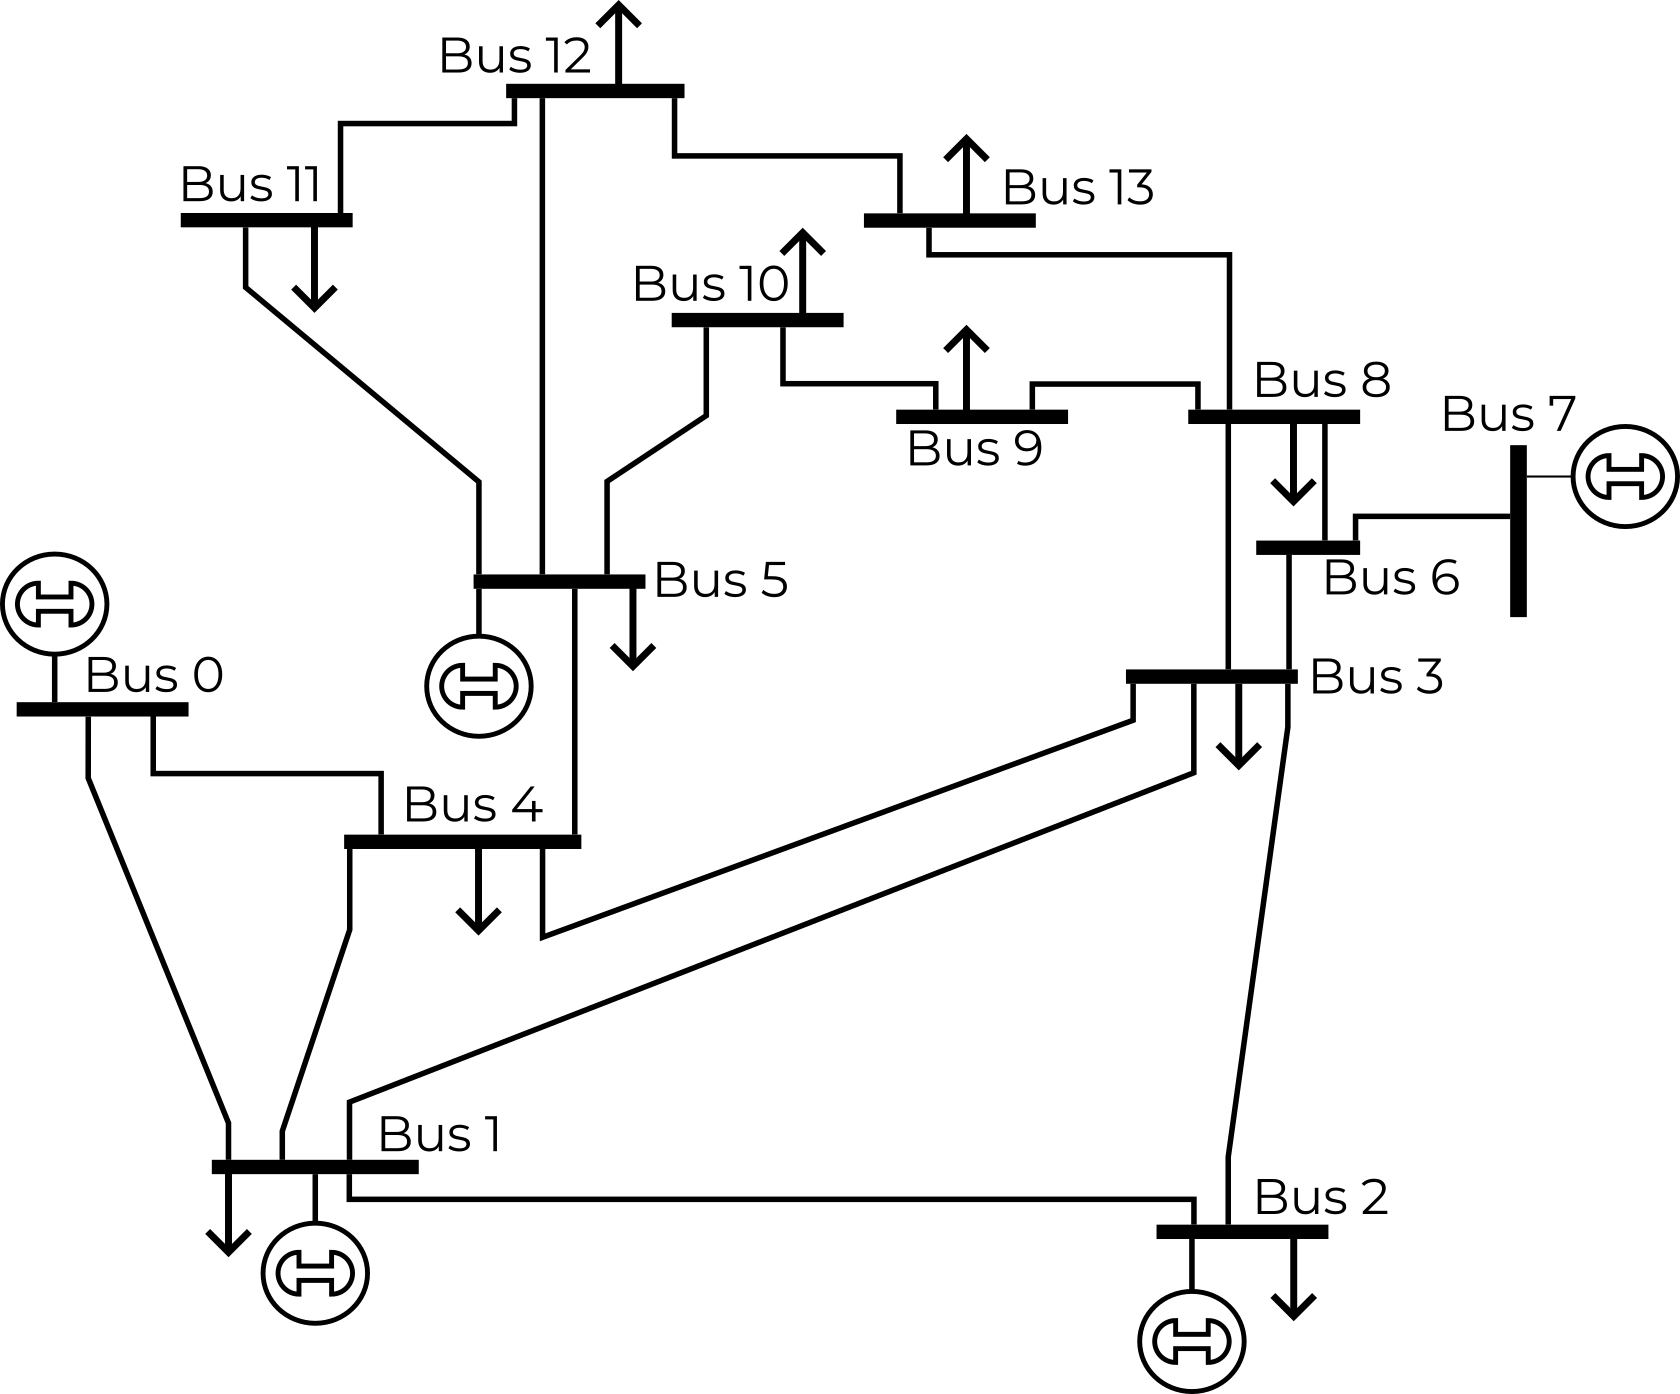
\includegraphics[width=\linewidth]{images/global_methods/base_14_bus.png}
    \end{subfigure}
    \begin{subfigure}[t]{0.4\linewidth}
        \centering
        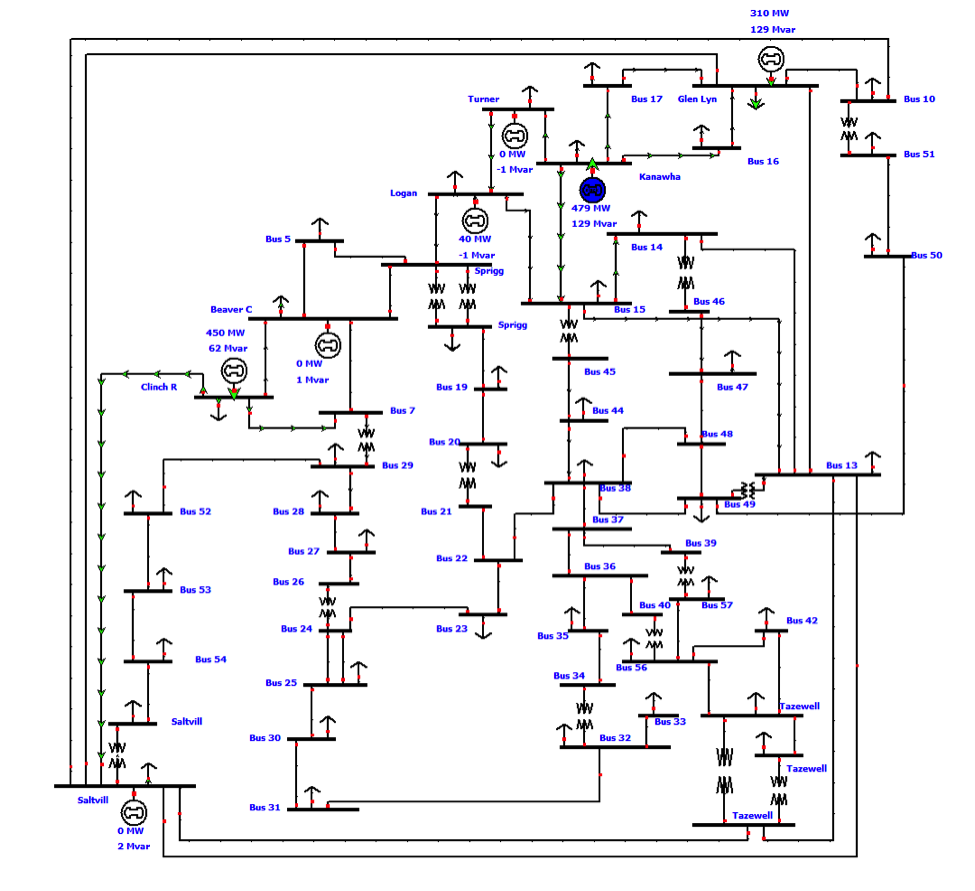
\includegraphics[width=\linewidth]{images/global_methods/IEEE57.png}
    \end{subfigure}%
    \caption{Example 14- and 57-bus electricity transmission networks~\cite{illinoiscenterforasmarterelectricgridIEEE57BusSystem}.}
    \label{ch:corl:fig:networks}
\end{figure}

A high-level comparison of RADIUM with existing methods is shown in Figs.~\ref{ch:corl:fig:nonvision_results} and~\ref{ch:corl:fig:convergence:nonvision}; in this section, we provide a more detailed comparison between RADIUM and prior optimization-based methods that are the state-of-the-art for this SCOPF problem~\cite{dontiAdversariallyRobustLearning2021} (the comparison with \ltc{} is not shown in thi section, since it is not able to solve the SCOPF problem).

\paragraph{Solution quality} To compare the quality of these methods' solutions, we use each method to optimize $10$ candidate designs and predict $10$ failure modes using Algorithm~\ref{ch:corl:alg:adv_diffusion}. We then select the design that achieves the highest likelihood according to Eq.~\eqref{ch:corl:eq:repair_logprob_tempered}, then use one additional round to sample new failure modes that attack the chosen design. The maximum cost across these final predicted failure modes provides a measure of each algorithm's confidence in its solution. We then compare the performance on these predicted failure modes to the maximum cost observed on a test set of $10^6$ exogenous parameters sampled randomly from the prior $p_{y, 0}$. Fig.~\ref{ch:corl:fig:scopf_comparison:14_bus} shows the predicted and observed costs for each method on the IEEE 14-bus test case. The prediction-and-mitigation process took \SI{30.5}{s} for \gdr{}, \SI{61.5}{s} for \gda{}, \SI{111.5}{s} for $R_0$, and \SI{141.7}{s} for $R_1$ (including the cost of JAX just-in-time compilation).

\begin{figure}[tb]
    \centering
    \begin{subfigure}[t]{0.45\linewidth}
        \centering
        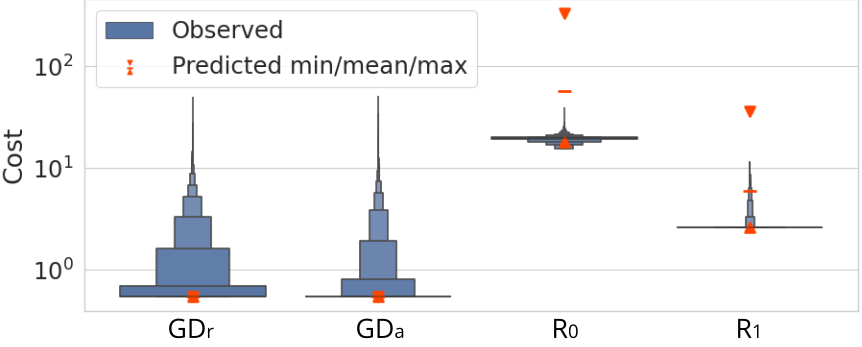
\includegraphics[width=\linewidth]{images/global_methods/14_bus_comparison.png}
        \caption{14-bus network}\label{ch:corl:fig:scopf_comparison:14_bus}
    \end{subfigure}
    \begin{subfigure}[t]{0.45\linewidth}
        \centering
        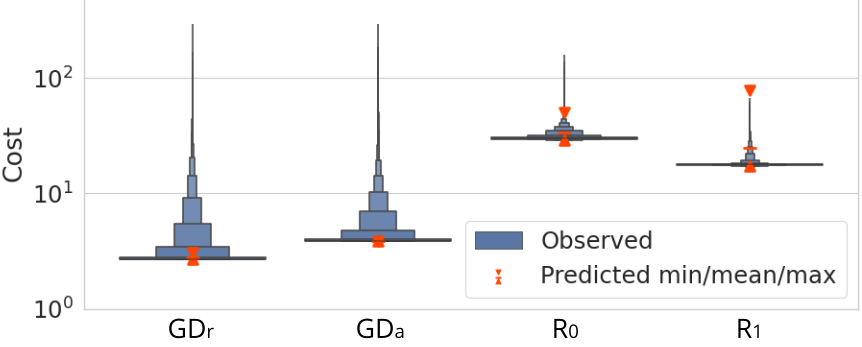
\includegraphics[width=\linewidth]{images/global_methods/57_bus_comparison.png}
        \caption{57-bus network}\label{ch:corl:fig:scopf_comparison:57_bus}
    \end{subfigure}
    \caption{Comparison of our method with baselines for failure prediction and mitigation on power transmission networks. Red markers show the maximum, mean, and minimum-cost failure modes predicted by each method after optimizing the design, while the box plot shows the distribution of costs on a test set of $10^6$ random failures.}
    \label{ch:corl:fig:scopf_comparison}
\end{figure}

We can assess these methods in two ways: by the quality of the optimized design and by the quality of the predicted failure cases. The two optimization-based methods, \gda{} and \gdr{}, find solutions with the lowest best-case cost, but their solutions are not robust. Not only do these methods find solutions that are susceptible to a heavy tail of failures, but they are overconfident and fail to predict those failures (instead predicting that all 10 candidate failures will be successfully mitigated). In contrast, $R_0$ is not overconfident (it successfully predicts failure modes that match the range of the empirical failure distribution), but it finds a solution that is 10 times costlier than those found by $R_1$. Only $R_1$ is able to find a robust, low-cost solution without being overconfident.

Once we have a robust design optimized using our method, we can examine the predicted failure modes to understand the remaining ways in which our design might fail. Of the 10 failure modes predicted by $R_1$, 4 include attacks on the transmission line connecting the generator at bus 7 to the rest of the network (this was the most commonly attacked line). Interestingly, of these 4 attacks, only one (shown in Fig.~\ref{ch:corl:fig:predicted_failure_modes}) is able to cause a violation of the voltage stability constraints. It is only by fully disconnecting the generator at bus 7 (dotted red line) and partially impairing the line between buses 1 and 4 (solid red; $15\%$ impairment) that we see the voltage drop at several buses (shown in orange). This information about potential failure modes can be very useful to system designers; in this example, the designer may choose to focus monitoring and infrastructure hardening efforts on the two affected lines.

\begin{figure}[tb]
    \centering
    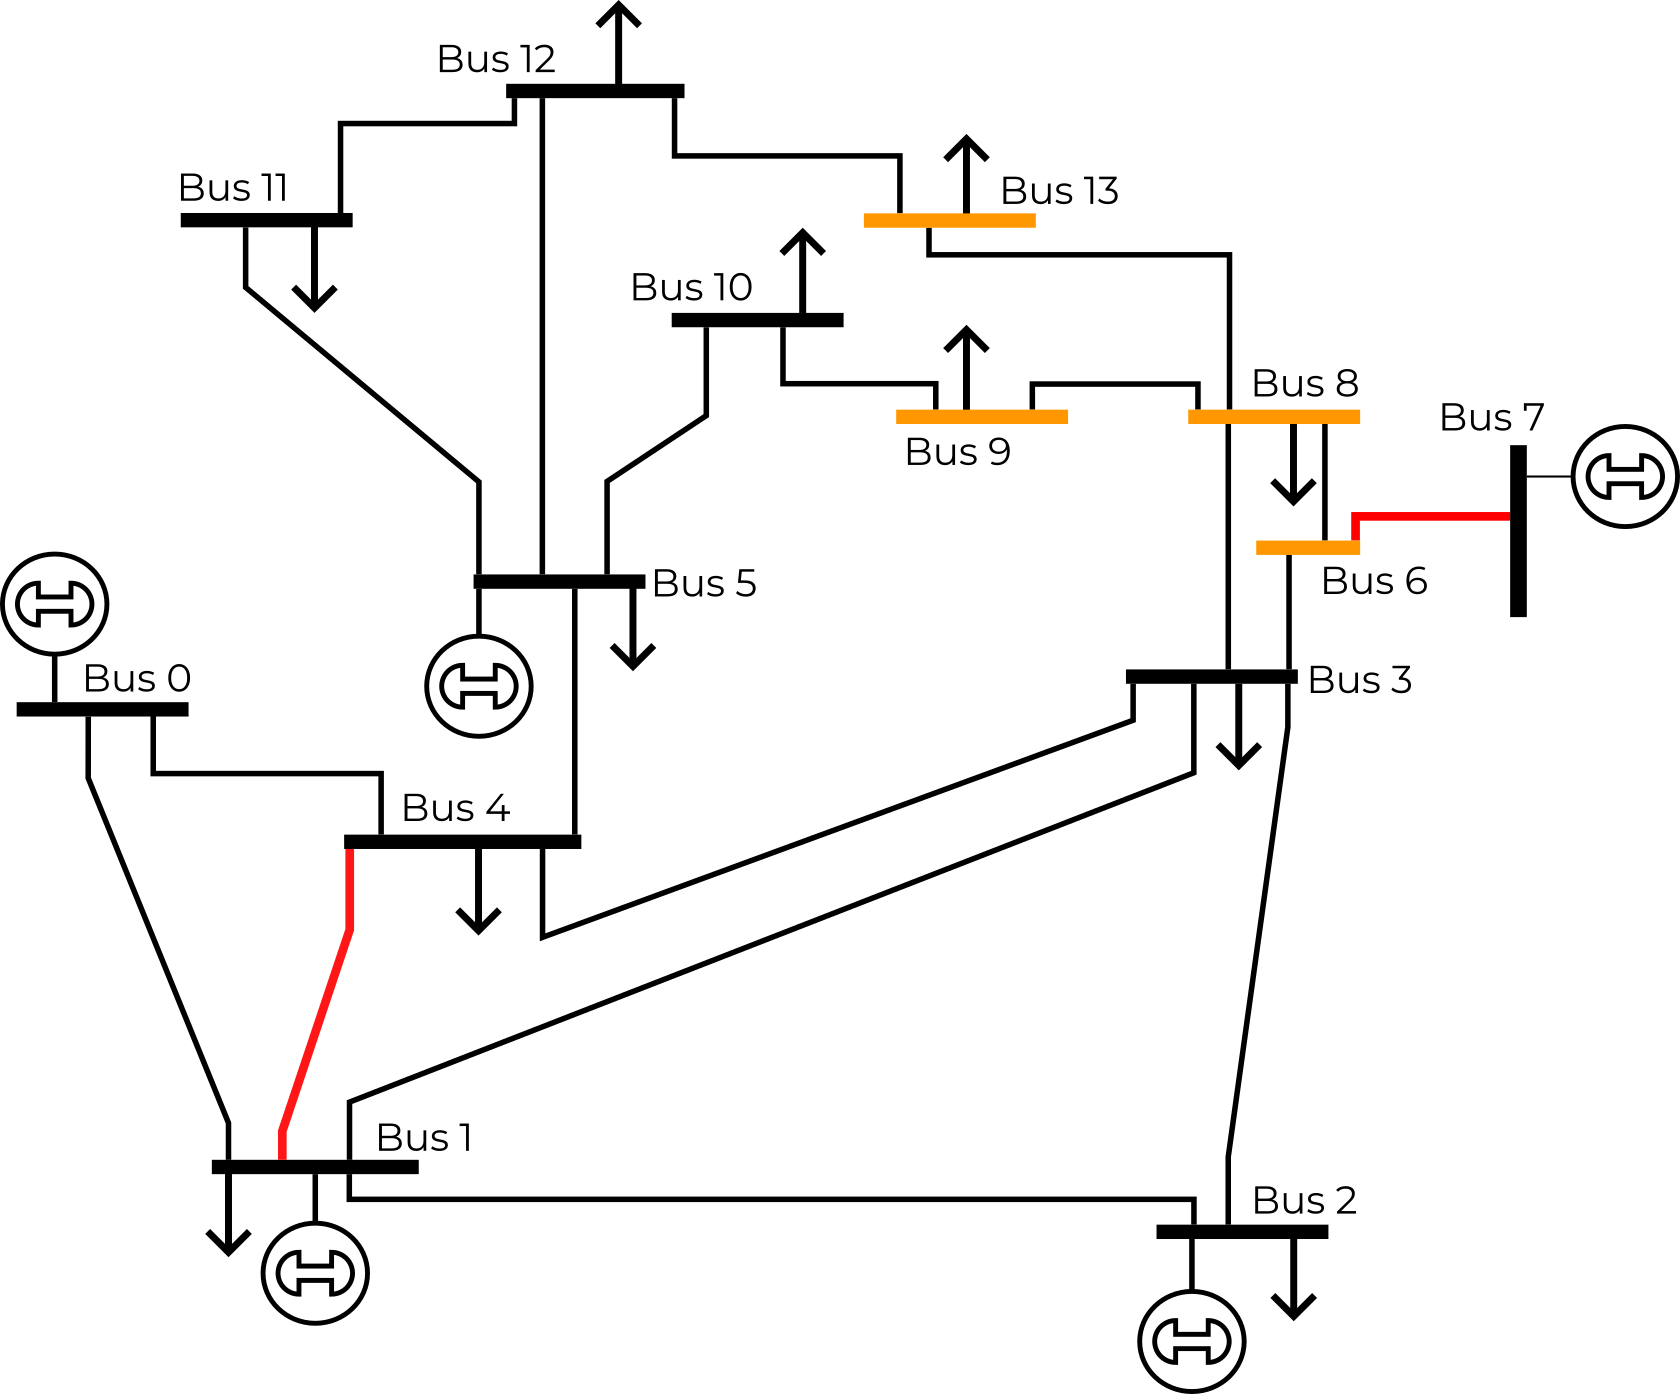
\includegraphics[width=0.4\linewidth]{images/global_methods/predicted_failure_modes.png}
    \caption{The only predicted failure modes (of 10 candidates) that causes violation of voltage constraints on the 14-bus transmission network, using the optimized design found using $R_1$. Fully disconnecting the generator at bus 7 (dotted red line) is not enough; other predicted failures include this outage but do not cause a constraint violation. It is only by additionally impairing the line between buses 1 and 4 that the voltage constraint is violated at the buses shown in orange.}
    \label{ch:corl:fig:predicted_failure_modes}
\end{figure}

To understand the scalability of our approach, we repeat this experiment on a larger 57-bus network with 80 transmission lines. All hyperparameters were the same except for the step size for exogenous parameters, which was reduced to $10^{-3}$. The results are shown in the bottom panel of Fig.~\ref{ch:corl:fig:scopf_comparison:14_bus}; we see that $R_1$ continues to not only find a robust solutions (with a relatively light tail of failures) but also accurately predicts the range of possible failure modes ($R_0$ does not explore the full failure space in this case). Running \gdr{} on this example takes \SI{406.2}{s}, \gda{} takes \SI{803.4}{s}, $R_0$ takes \SI{1002.3}{s}, and $R_1$ takes \SI{1438.5}{s}.

\paragraph{Convergence rate} From comparing solution quality, there is a clear separation between the sampling- and optimization-based methods, with sampling able to find more robust designs and more accurately cover the range of possible failures (although gradient-based sampling finds higher-quality solutions than gradient-free sampling in both cases). A natural next question is how quickly these methods converge to a solution.

To measure the relative convergence rate of \gdr{}, \gda{}, $R_0$, and $R_1$, we measure the 99\textsuperscript{th} percentile cost $J$ of the candidate design $[x]_i$ with the highest log likelihood~\eqref{ch:corl:eq:repair_logprob_tempered} on a test set of 1000 exogenous parameters sampled randomly from the prior. The convergence of this test-set performance as a function of the number of sampling rounds is shown in Fig.~\ref{ch:corl:fig:power_training_curves} for both the 14- and 57-bus networks.

\begin{figure}[tb]
    \centering
    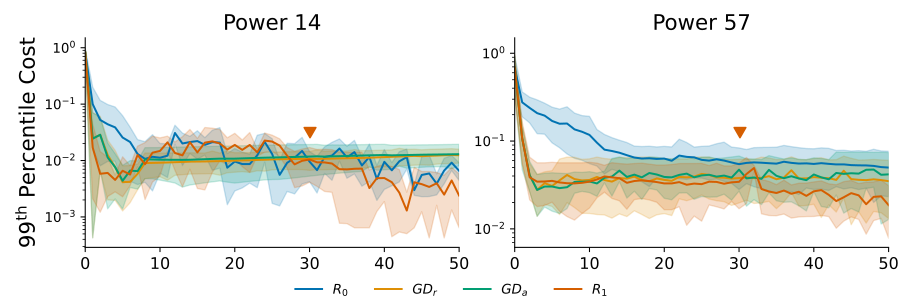
\includegraphics[width=\linewidth]{images/corl/power_convergence.png}
    \caption{Comparison of convergence rates of different methods on 14- (left) and 57-bus (right) power networks, showing the 99\textsuperscript{th} percentile cost of the best design after each round. The {\color{orange} $\blacktriangledown$} symbol indicates the start of quenching for $R_1$.}
    \label{ch:corl:fig:power_training_curves}
\end{figure}

There are two important conclusions to be drawn from comparing the convergence rates in Fig.~\ref{ch:corl:fig:power_training_curves}. The first is that the gradient-based methods, \gdr{}, \gda{}, and $R_1$, converge faster than gradient-free $R_0$. Although the SCOPF problem (as well as ACOPF, the non-adversarial version) are non-convex optimization problems, there are known convex relaxations~\cite{huangReviewConvexificationMethods2019}, and gradient descent-based methods have been shown to work well for finding local optima~\cite{dontiAdversariallyRobustLearning2021,dontiDC3LearningMethod2021}, so the good performance of gradient-based methods is not surprising.

The second important conclusion from Fig.~\ref{ch:corl:fig:power_training_curves} is the importance of quenching $R_1$ on this problem (i.e. disabling the stochastic part of the sampling algorithm and taking a few gradient descent steps during the final rounds). Prior to quenching, $R_1$ converges to a solution with similar 99\textsubscript{th} percentile cost as \gdr{} and \gda{}, but after quenching (in the last 20 rounds), $R_1$ is able to find a solution with a much lower cost. This is likely because of the constraints on $P$, $Q$, and $|V|$ in the SCOPF problem; sampling based methods may struggle to exactly satisfy constraints like these, as $MALA$ and $RMH$ are constantly injecting noise into the solution, and so running a few steps of gradient descent on $\theta$ towards the end of the repair process likely helps drive constraint violations to zero by converging to the local minima nearest to the solutions explored by the sampling process. The fact that $R_1$ converges to a lower-cost solution than \gdr{} or \gda{}, despite running the same gradient-based optimization process during the quenching phase, suggests that the improved exploration of designs and failures due to sampling provides an advantage over pure optimization-based methods on this problem.

\subsection{Case study on multi-agent path planning}

We return to the search problem used as a baseline in Section~\ref{ch:corl:experiments}, where a team of seeker robots must cover a region to detect a set of hiders. The simulation environment includes $n_{seek}$ seeker robots and $n_{hide}$ hider robots. Each robot is modeled using single-integrator dynamics and tracks a pre-planned trajectory using a proportional controller with saturation at a maximum speed chosen to match that of the Robotarium platform~\cite{wilsonRobotariumGloballyImpactful2020}. The trajectory $\vec{x}_i(t)$ for each robot is represented as a Bezier curve with 5 control points $\vec{x}_{i, j}$,
\begin{align*}
    \vec{x}_i(t) = \sum_{j=0}^4 \binom{4}{j}(1-t)^{4-j}t^j \vec{x}_{i, j}
\end{align*}

The design parameters are the 2D position of the control points for the trajectories of the seeker robots, while the exogenous parameters are the control points for the hider robots. The prior distribution for each set of parameters is uniform over the width and height of the Robotarium arena ($\SI{3.2}{m}\times\SI{2}{m}$).

We simulate the behavior of the robots tracking these trajectories for \SI{100}{s} with a discrete time step of \SI{0.1}{s} (including the effects of velocity saturation that are observed on the physical platform), and the cost function is
\begin{align*}
    J = \sum_{i=1}^{n_{hide}}\pn{\mathop{\widetilde{\min}}_{t = t_0, \ldots, t_{n}} \pn{\mathop{\widetilde{\min}}_{j=1, \ldots, n_{seek}}\norm{\vec{p}_{hide, i}(t) - \vec{p}_{seek, j}(t)} - r}}
\end{align*}
%
where $r$ is the sensing range of the seekers (\SI{0.5}{m} for the $n_{seek} = 2$ case and \SI{0.25}{m} for the $n_{seek}=3$ case); $\widetilde{\min}(\circ) = -\frac{1}{b}\text{logsumexp}(-b\ \circ)$ is a smooth relaxation of the element-wise minimum function where $b$ controls the degree of smoothing ($b=100$ in our experiments); $t_0, \ldots, t_{n}$ are the discrete time steps of the simulation; and $\vec{p}_{hide, i}(t)$ and $\vec{p}_{seek, j}(t)$ are the $(x, y)$ position of the $i$-th hider and $j$-th seeker robot at time $t$, respectively. In plain language, this cost is equal to the sum of the minimum distance observed between each hider and the closest seeker over the course of the simulation, adjusted for each seeker's search radius.

We deploy the optimized hider and seeker trajectories in hardware using the Robotarium multi-robot platform~\cite{wilsonRobotariumGloballyImpactful2020} (we use 3 seekers and 5 hiders, since we had difficulty testing with more agents in the limited space). We first hold the search pattern (design parameters) constant and optimize evasion patterns against this fixed search pattern, yielding the results shown on the left in Fig.~\ref{fig:hw_experimental_results} where the hiders easily evade the seekers. We then optimize the search patterns using our approach (with $K=100$ rounds and $M=10$ substeps per round, taking \SI{41}{s}), yielding the results on the left where the hiders are not able to evade the seekers. Trajectories for the hiders and seekers were planned offline and then tracked online using linear trajectory-tracking controllers.

\begin{figure}[tb]
    \centering
    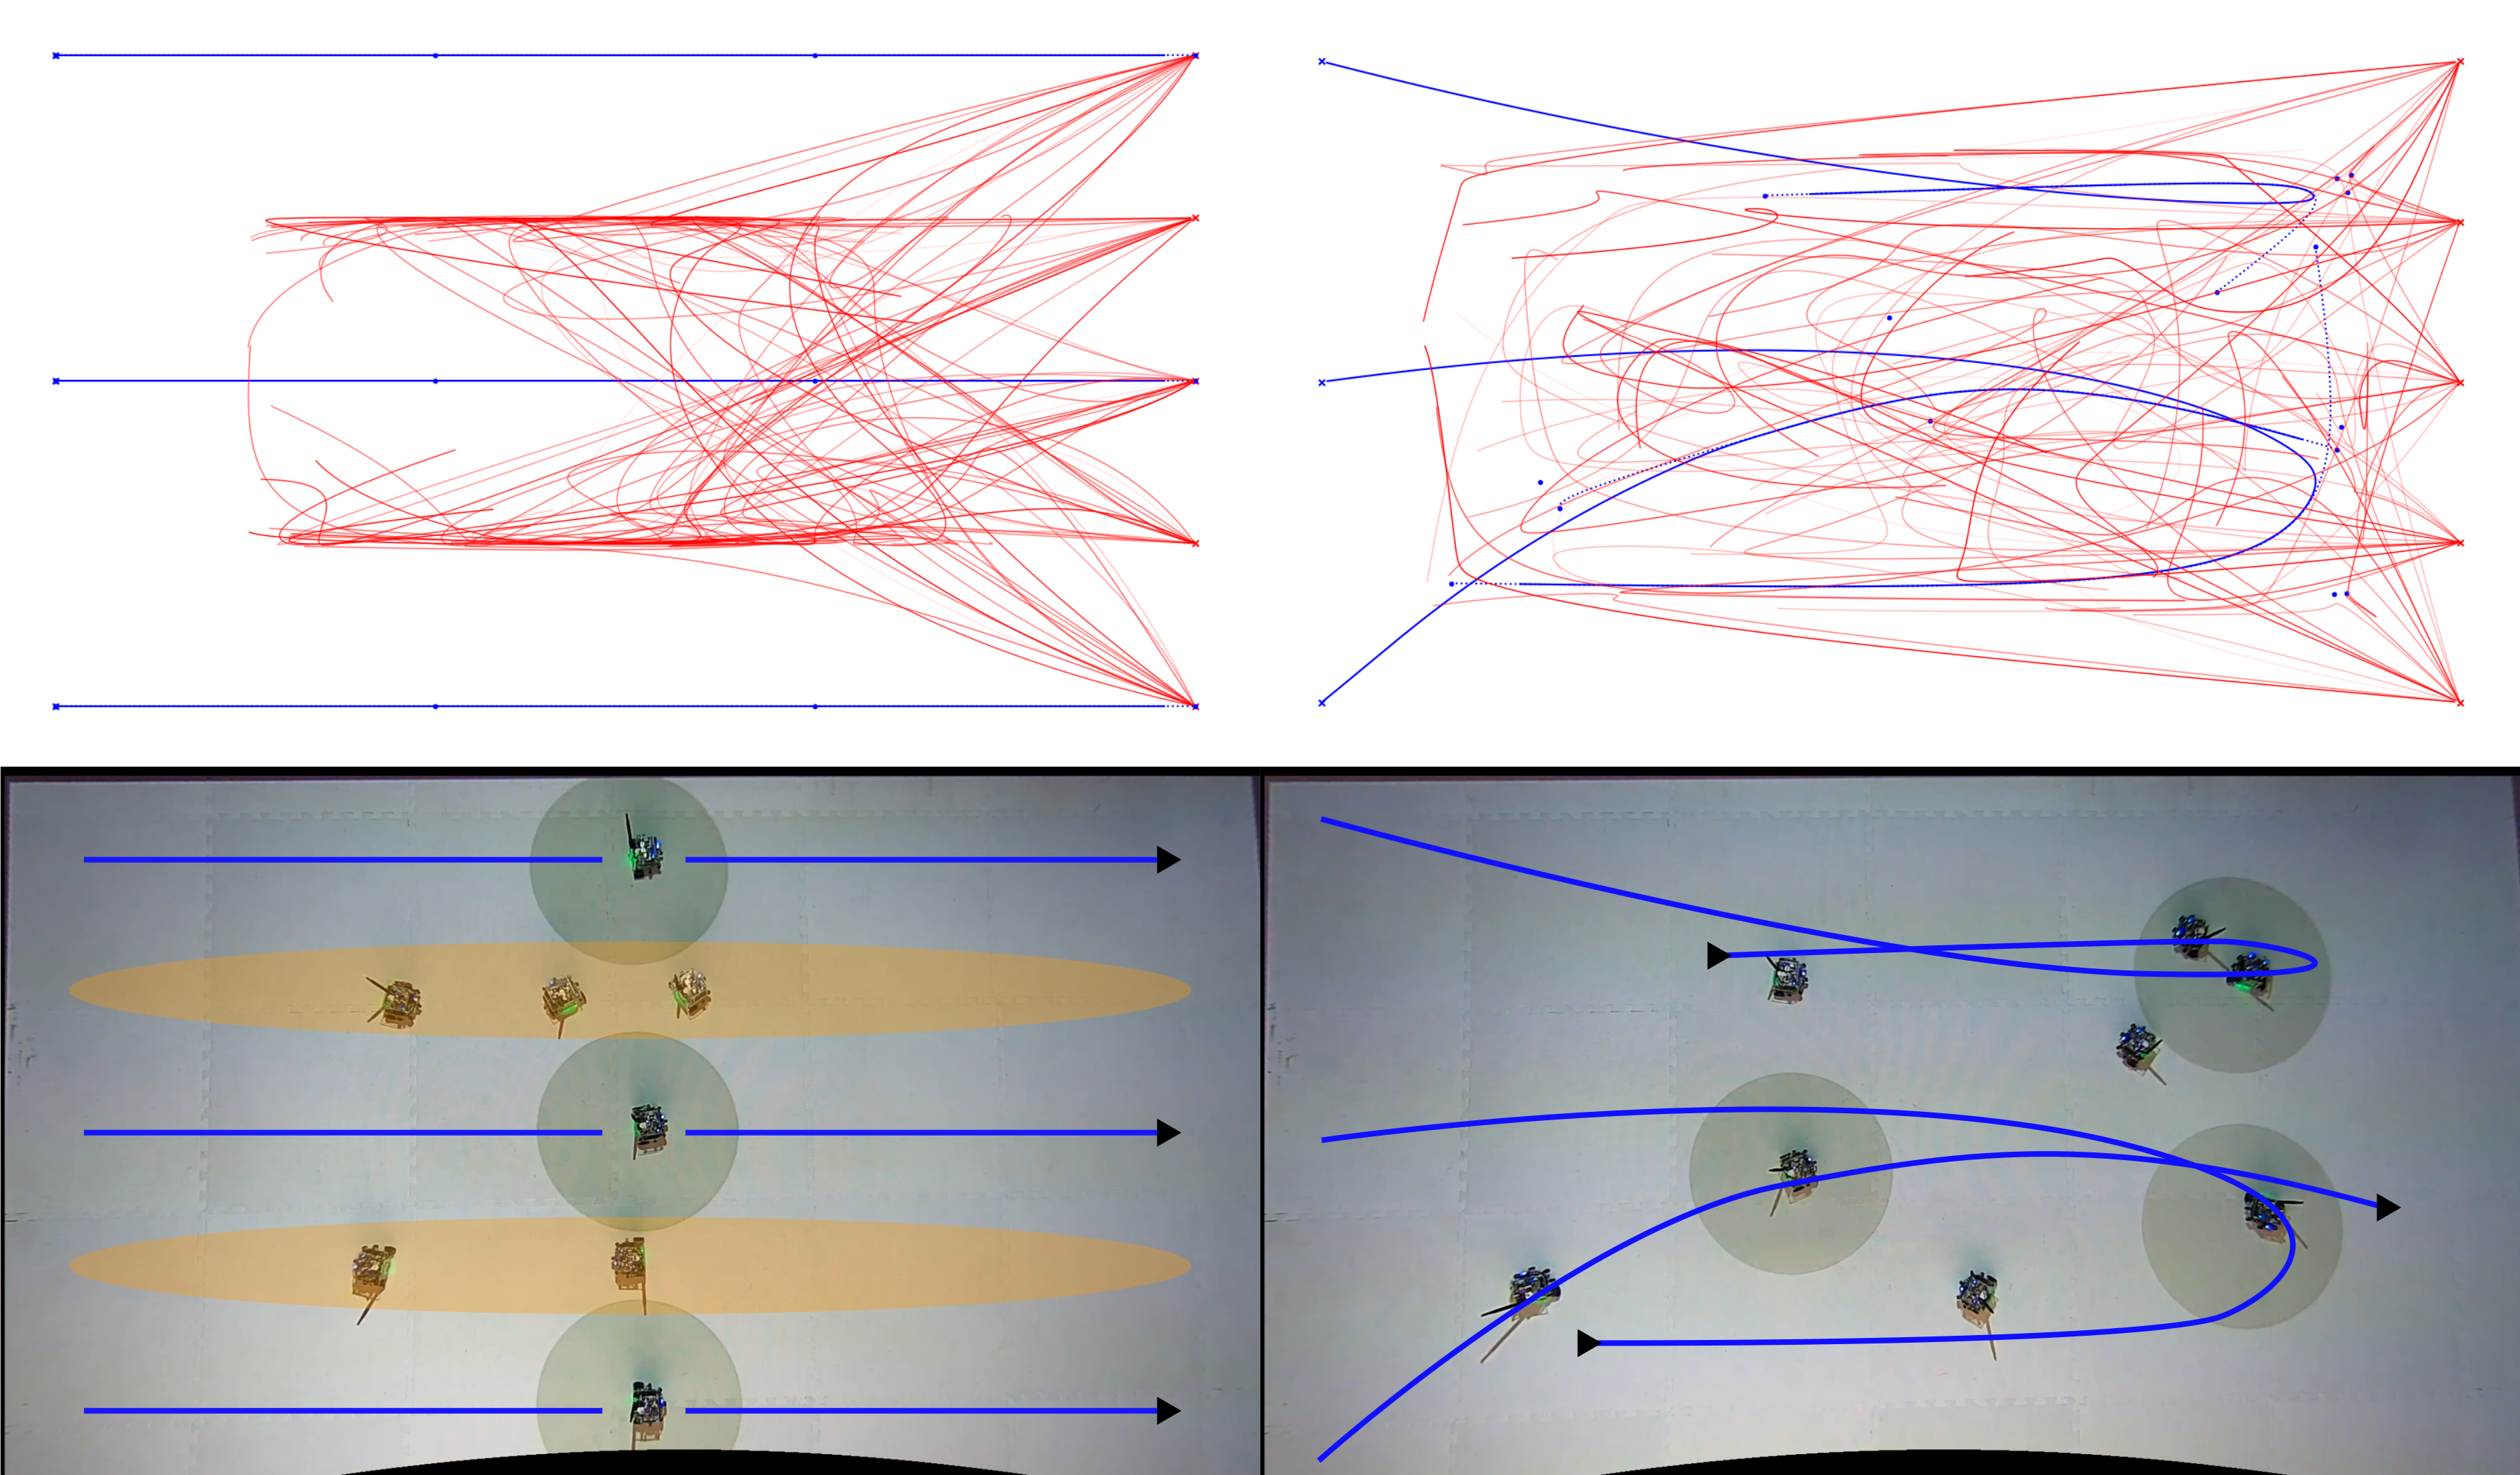
\includegraphics[width=\linewidth]{images/corl/hw_results.png}
    \caption{(Left) HW results for search-evasion with 5 hiders and 3 seekers, showing an initial search pattern (seeker trajectories; blue) and predicted failure modes (hider trajectories; red). (Right) HW results for an optimized search pattern leaves fewer hiding places. The top row shows the predicted failure modes (i.e. hider trajectories), while the bottom row shows a snapshot from hardware executions of these trajectories.}
    \label{fig:hw_experimental_results}
\end{figure}

Although the gap between simulation and reality is not particularly large in this case, there are effects present in the hardware system that we did not model in our simulator (e.g. the collision-avoidance safety filter used by the Robotarium). Despite this small gap, this case study serves as a useful proof-of-concept for transferring optimized designs from simulation to hardware.
%
% In the next case study, we will demonstrate the transfer of failure modes and repaired designs in a much more challenging environment with vision in the loop.

% \subsection{Case study on vision-in-the-loop control of a model racecar}

% TODO

\section{Conclusion \& Limitations}

In this chapter, we close several key gaps in the prior work on adversarial design optimization. In particular, we reframe the adversarial optimization problem studied in Chapter~\ref{ch:iros} as a inference problem solved by sampling from specially constructed pseudo-posterior distributions. This reformulation brings three key advantages. First, it allows us to use gradient-based sampling algorithms that are robust to high-variance or poorly conditioned gradients that would otherwise cause a gradient-based optimization algorithm to diverge. Second, our stochastic sampling-based methods is able to avoid local minima that cause gradient-based optimizers to get stuck. Finally, since our method focused on sampling a range of high-severity failures, rather than finding a single most-severe failure, we are able to find a much more diverse set of counterexamples than prior optimization-based methods. Ultimately, these diverse counterexamples allow us to optimize against a more challenging curriculum of failure modes, leading to more robust designs.

We apply our approach to a range of robotics and cyberphysical control problems, demonstrating how the use of gradients from differentiable simulation and rendering can help accelerate convergence. However, we acknowledge that a differentiable simulation environment is not always available, and that substantial engineering effort can be required to develop such a simulator. Because of this difficulty, and because simulators of certain phenomena (e.g., contact~\cite{huDiffTaichiDifferentiableProgramming2019} and rendering with occlusion~\cite{zhaoPhysicsbasedDifferentiableRendering2020}) can yield inaccurate gradients if care is not taken, we build graceful degradation into our approach, providing a gradient-free version of our algorithm that can be used when gradients are not available. When gradient quality is poor, we find empirically that the acceptance rate of $R_1$ will fall to zero, which provides feedback to the user to either improve their differentiable simulator or switch to $R_0$ (which we find outperforms gradient-free baselines on the benchmark problems studied in this chapter).

Although the RADIUM framework developed in this chapter closes a number of important technical gaps from previous chapters, there are several limitations that remain to be addressed. First, these methods rely on a manually-specified cost function to define failures. For some complex systems, it may be difficult to specify an appropriate cost function \textit{a priori}, and doing so may lead our method to focus only on those failures defined by the cost function, preventing the discovery of other undesirable behaviors. Second, RADIUM relies entirely on simulation for discovering failures and repairing designs; although we can transfer RADIUM's designs and predicted failures from simulation to hardware, there is no immediately obvious way to feed the results of hardware experiments back into RADIUM. In the next chapter, we introduce a method for data-driven failure analysis that allows us to close the loop between simulation and real-world data, while avoiding the need for a hand-specified cost function.
